% !TeX root = ../main.tex
% 原始章节：08-verification-and-implementation.Rmd

\chapter{芯片实现与验证}\label{chap:08-verification-and-implementation}

\section{需求分析：确定处理器芯片的目标应用}\label{sec:08-verification-and-implementation-001}

处理器芯片的目标应用通常取决于其架构、性能和特定目标设计。如图\ref{fig:08-cpu-application}是几种常见的目标应用。

\begin{figure}[htbp]
  \centering
  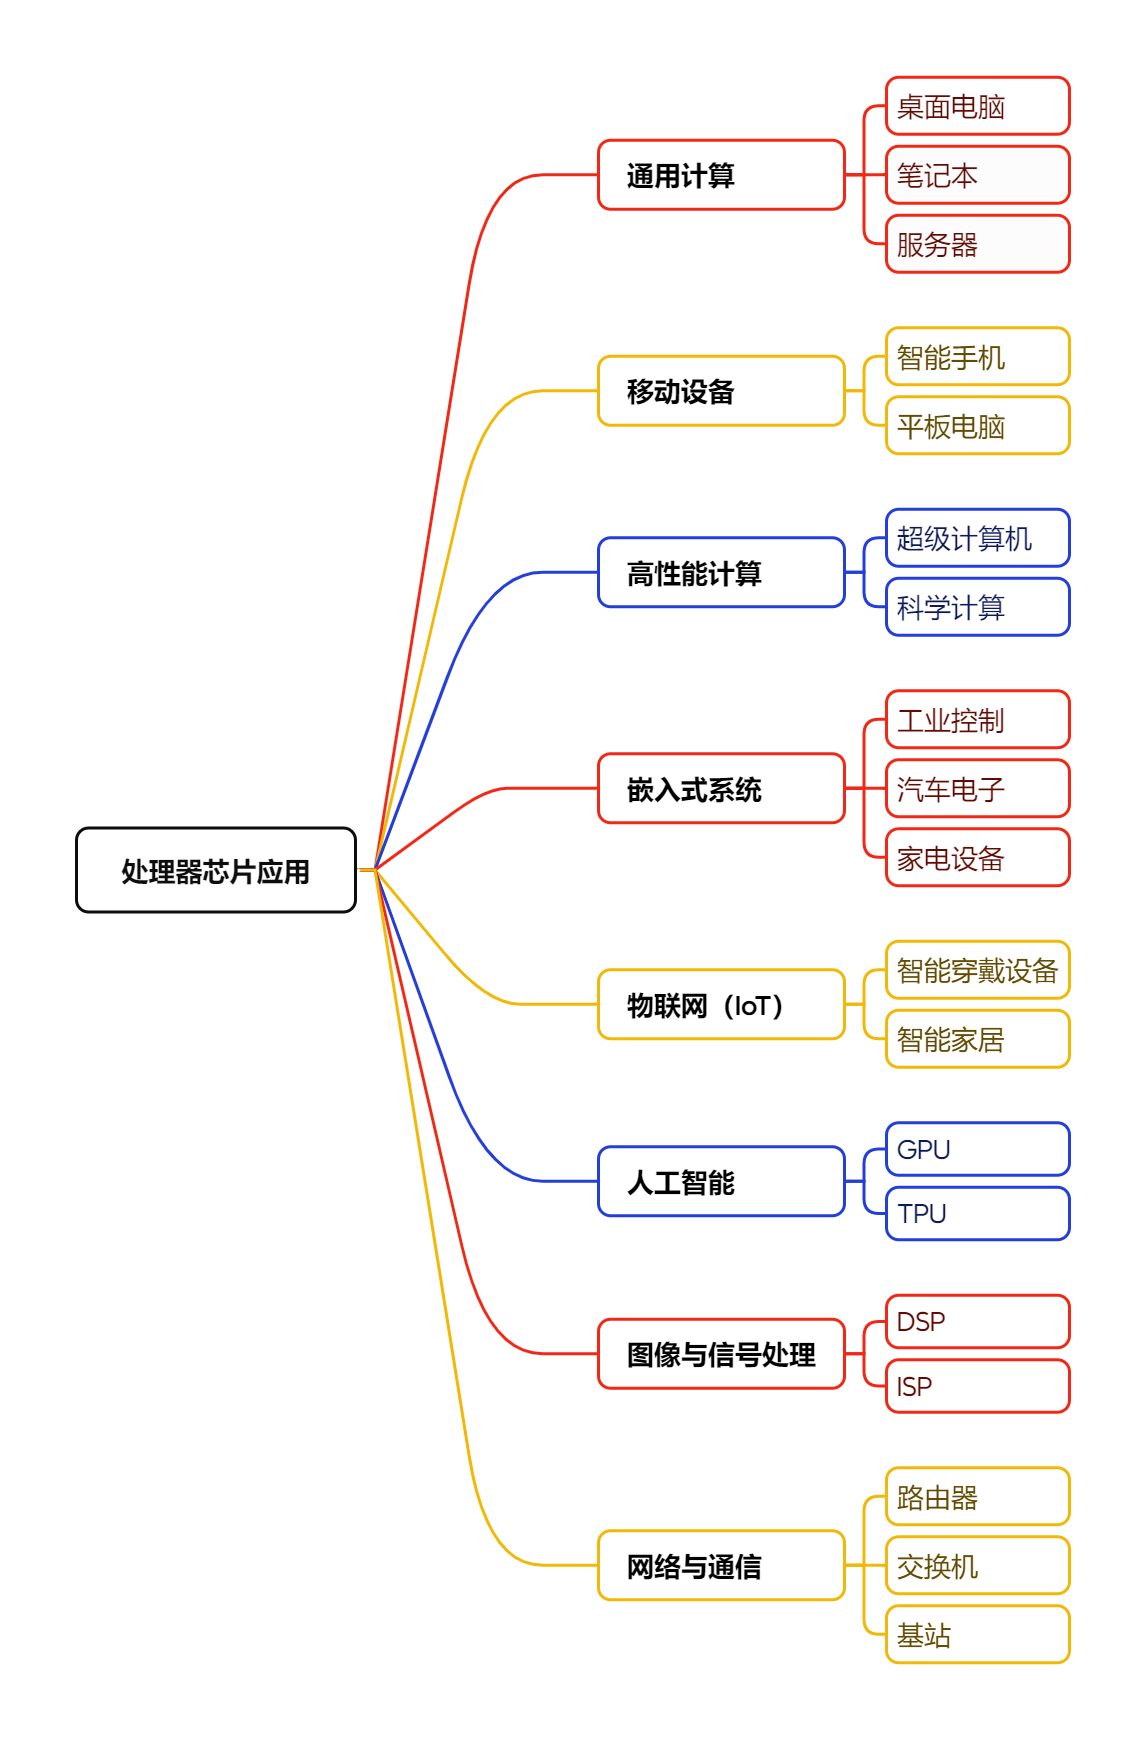
\includegraphics[width=0.3\linewidth]{assets/08/处理器芯片应用.png}
  \caption{处理器芯片目标应用}
  \label{fig:08-cpu-application}
\end{figure}

\begin{itemize}
\item
  1.通用计算：适用于桌面电脑、笔记本、服务器等。此类处理器需要具备较强的多任务处理能力和高效能以应对各种计算任务。
\item
  2.移动设备：专为智能手机、平板电脑等移动设备设计。此类处理器需要在低功耗的前提下提供较高的性能，以延长电池寿命并支持多媒体处理、通信等功能。
\item
  3.嵌入式系统：用于工业控制、汽车电子、家电等领域的嵌入式系统。嵌入式处理器通常要求高可靠性、实时性和低功耗。
\item
  4.高性能计算（HPC）：面向超级计算机、科学计算等需要极高计算能力的领域。此类处理器通常集成多核、多线程，并支持并行计算和高速数据传输。
\item
  5.人工智能（AI）和机器学习：专为加速神经网络、深度学习等AI任务设计的处理器，如GPU、TPU等。它们通常包含大量并行处理单元，用于处理大规模数据和复杂算法。
\item
  6.物联网（IoT）：用于智能家居、可穿戴设备、环境监测等IoT设备。此类处理器要求极低功耗、较小体积，并能与各种传感器和网络接口进行高效交互。
\item
  7.图像与信号处理：专用于图像处理、视频编码解码、音频处理等领域的处理器，如DSP（数字信号处理器）和ISP（图像信号处理器）。这些处理器通常优化了特定的数据处理算法。
\item
  8.网络与通信：用于路由器、交换机、基站等网络设备的处理器，通常强调高速数据处理、低延迟和高吞吐量。
\end{itemize}

本处理器芯片主要作为教学目的，其coremark测试得分为451，其性能可对标STM32L552（coremark得分443）。考虑到性能、功耗、大小、外设等因素，该芯片可应用于嵌入式设备（如类似树莓派等）。

\section{确定芯片整体规格}\label{sec:08-verification-and-implementation-002}

首先，我们需清晰界定CPU将主要服务于哪些嵌入式场景，如物联网设备、教育学习机、工业自动化控制、数字标牌等。根据这些场景，明确CPU的功能需求（如多任务处理能力、实时性要求）、性能需求（处理速度、响应时间）、功耗限制（长时间运行下的低功耗）、接口需求（与外部传感器的连接、显示接口等）。

针对嵌入式设备特有的低功耗、高集成度、稳定性要求，进行针对CPU及SOC的技术可行性分析:

\begin{itemize}
\tightlist
\item
  \textbf{性能规格}：

  \begin{itemize}
  \tightlist
  \item
    主频与核心数：根据应用场景选择适中的主频与核心数，确保高效处理同时控制功耗。本CPU设计是单核CPU。
  \item
    缓存大小：合理配置缓存，以加速数据访问，减少内存延迟。经过设计需求，确定指令缓存以及数据缓存设置为8KB。
  \item
    运算能力：针对特定算法（如加密、图像处理）优化运算单元。
  \item
    AXI4总线：具有高性能、高带宽、可扩展性与灵活性强等特点，在许多外设接口都可使用AXI4总线进行与CPU的交互。
  \end{itemize}
\item
  \textbf{功耗规格}：

  \begin{itemize}
  \tightlist
  \item
    工作与待机功耗：设计低功耗模式，确保长时间运行时的能效比。本芯片板级功耗控制在3W以内。
  \item
    动态功耗管理：集成智能功耗管理机制，根据负载自动调节功耗。
  \end{itemize}
\item
  \textbf{外设接口规格}：

  \begin{itemize}
  \tightlist
  \item
    GPIO接口：支持多通道输入输出，便于连接各类传感器和执行器。本SOC考虑芯片引脚受限等因素，将GPIO与其他功能接口共用（如USB）。
  \item
    高速通信接口：集成USB 控制器、Ethernet等标准通讯接口。
  \item
    低速通信接口：集成SPI、I2C、CDBUS、UART等接口，以适应不同通讯需求。
  \item
    音视频接口：自行设计HDMI、I2S等音视频接口。
  \end{itemize}
\item
  \textbf{存储接口规格}：

  \begin{itemize}
  \tightlist
  \item
    SDRAM内存控制器：支持SDRAM标准接口，确保数据处理速度的同时控制功耗。
  \item
    闪存接口：支持SPI，提供灵活的数据存储方案。
  \item
    SD CARD存储控制及接口控制
  \end{itemize}
\item
  \textbf{硬件加速器规格}：

  \begin{itemize}
  \tightlist
  \item
    图像处理单元：在本设计中想要CPU具有视频播放、图片查看等能力，因此加入了JEPG Decoder硬解码单元，支持硬件解码播放720P视频。
  \end{itemize}
\item
  \textbf{软件支持规格}：

  \begin{itemize}
  \tightlist
  \item
    处理器核心支持Linux内核以及U-Boot等多系统软件及应用软件。
  \end{itemize}
\end{itemize}

综合考虑以上规格内容，可以确定处理器芯片的性能、功耗、接口、软件支持等方面进行全面的分析。

\section{芯片的FPGA上板验证}\label{sec:08-verification-and-implementation-003}

芯片功能基本完整后/流片前需要进行完善的FPGA上板验证，FPGA开发流程和IC的开发流程相似，主要分为以下几个部分：

\begin{enumerate}
\def\labelenumi{\arabic{enumi}.}
\tightlist
\item
  设计输入，利用HDL输入工具、原理图输入工具或状态机输入工具等把所要设计的电路描述出来；
\item
  功能验证，也就是前仿真，利用Modelsim、VCS等仿真工具对设计进行仿真，检验设计的功能是否正确；常用的仿真工具有Model Tech公司的ModelSim，Synopsys公司的VCS，Cadence公司的NC-Verilog和NC-VHDL，Aldec公司的Active HDL VHDL/Verilog HDL等。仿真过程能及时发现设计中的错误，加快了设计进度，提高了设计的可靠性。（这一部分内容已经包含在\textbf{敏捷开发流程}中）
\item
  综合，综合优化是把HDL语言翻译成最基本的与或非门的连接关系（网表），并根据要求（约束条件）优化所生成的门级逻辑连接，输出edf和edn等文件，导给CPLD/FPGA厂家的软件进行实现和布局布线。常用的专业综合优化工具有Synplicity公司的synplify /Synplify Pro、Amplify等综合工具，Synopsys公司的FPGA Compiler II综合工具（Synopsys公司将停止发展FPGA Express软件，而转到FPGA Compiler II平台），Exemplar Logic公司出品的LeonardoSpectrum等综合工具。另外FPGA/CPLD厂商的集成开发环境也带有一些综合工具，如Xilinx的Vivado等。
\item
  布局布线，综合的结果只是通用的门级网表，只是一些门与或非的逻辑关系，与芯片实际的配置情况还有差距。此时应该使用FPGA/CPLD厂商提供的实现与布局布线工具，根据所选芯片的型号，进行芯片内部功能单元的实际连接与映射。这种实现与布局布线工具一般要选用所选器件的生产商开发的工具，因为只有生产者最了解器件内部的结构，如在ISE的集成环境中完成实现与布局布线的工具是Flow Engine。
\item
  时序验证，其目的是保证设计满足时序要求，即setup/hold time符合要求，以便数据能被正确的采样。时序验证的主要方法包括STA（Static Timing Analysis）和后仿真。在后仿真中将布局布线的时延反标到设计中去，使仿真既包含门延时，又包含线延时信息。这种后仿真是最准确的仿真，能较好地反映芯片的实际工作情况。仿真工具与综合前仿真工具相同。
\item
  生成并下载BIT或PROM文件，进行板级调试。
\end{enumerate}

下面我们介绍如何进行FPGA上版验证：

\textbf{Note:} 基于MegaSoC和百芯开发板的上板流程可以参考视频：\url{https://www.bilibili.com/video/BV1gXe8eUEmd}

\subsection{创建工程}\label{sec:08-verification-and-implementation-004}

通过双击桌面快捷方式或开始菜单的``Xilinx Design Tools→Vivado 2019.2''打开Vivado 2019.2，在界面上的``Quick Start''下选择``Create Project''，如图\ref{fig:08-vivado-start}所示。

\begin{figure}[htbp]
  \centering
  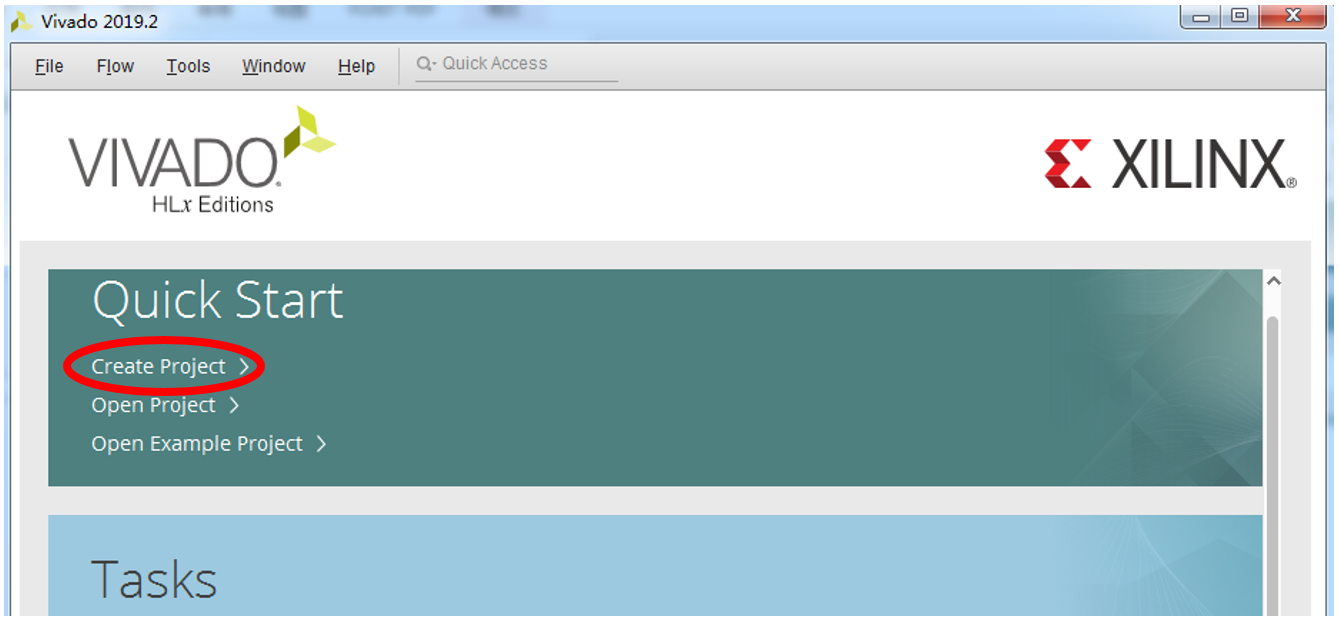
\includegraphics[width=1.0\linewidth]{assets/08/vivado_start.png}
  \caption{Vivado启动界面}
  \label{fig:08-vivado-start}
\end{figure}

这时即可新建工程向导，点击``Next''，如图\ref{fig:08-vivado-new}所示。

\begin{figure}[htbp]
  \centering
  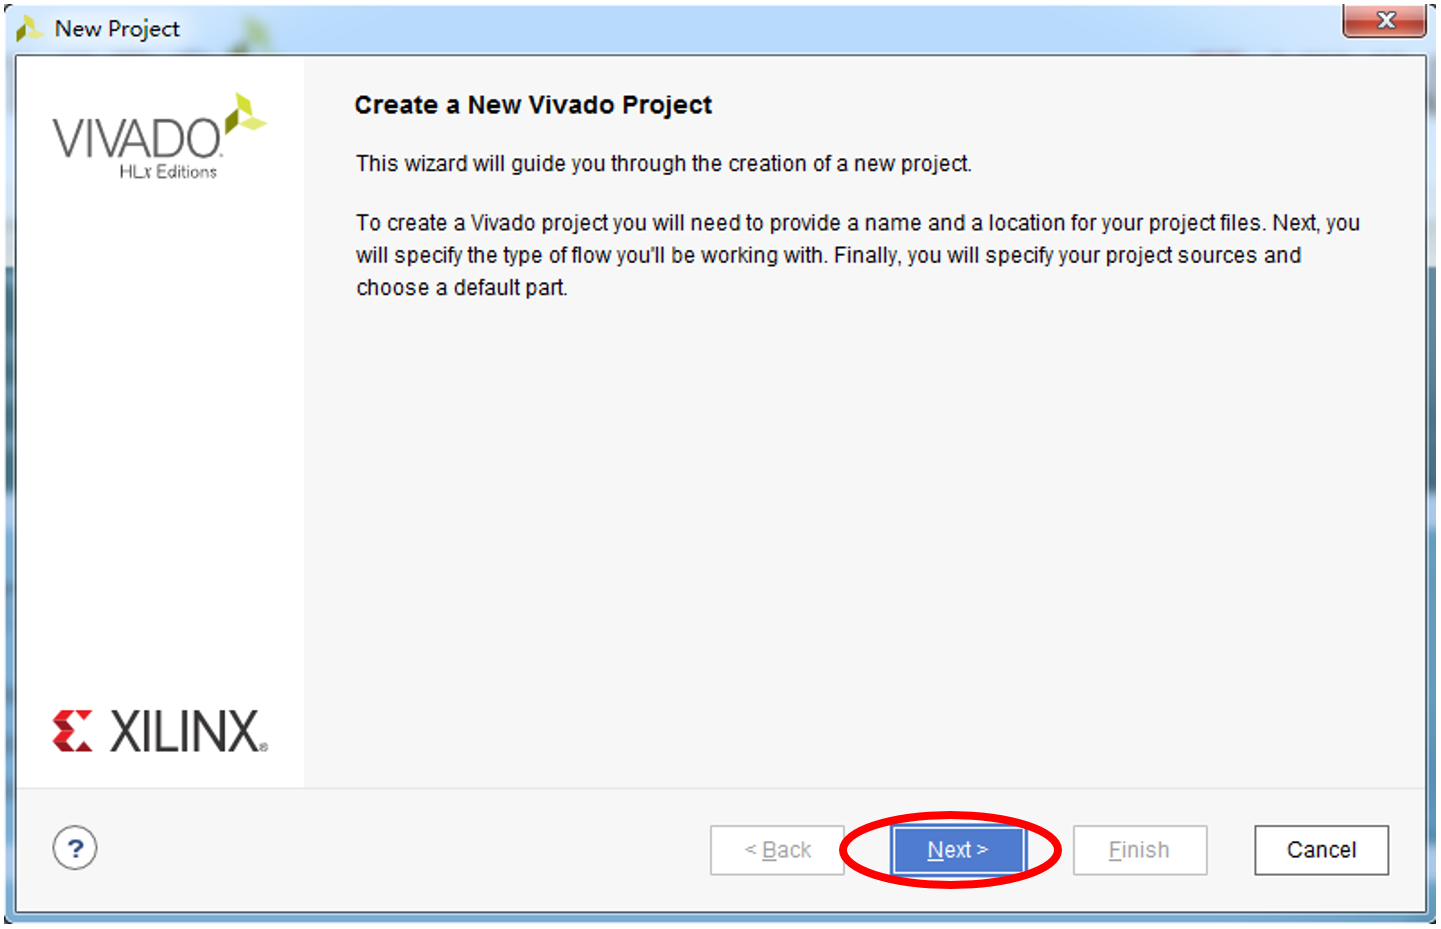
\includegraphics[width=1.0\linewidth]{assets/08/vivado_new_project_start.png}
  \caption{新建工程向导}
  \label{fig:08-vivado-new}
\end{figure}

在图\ref{fig:08-vivado-set-project-name}所示界面中输入工程名称，选择工程的存储路径，并勾选``Create project subdirectory''选项，为工程在指定存储路径下建立独立的目录。设置完成后，点击``Next''。（注意：工程名称和存储路径中不能出现中文字符和空格，建议工程名称以字母、数字、下划线来组成。）

\begin{figure}[htbp]
  \centering
  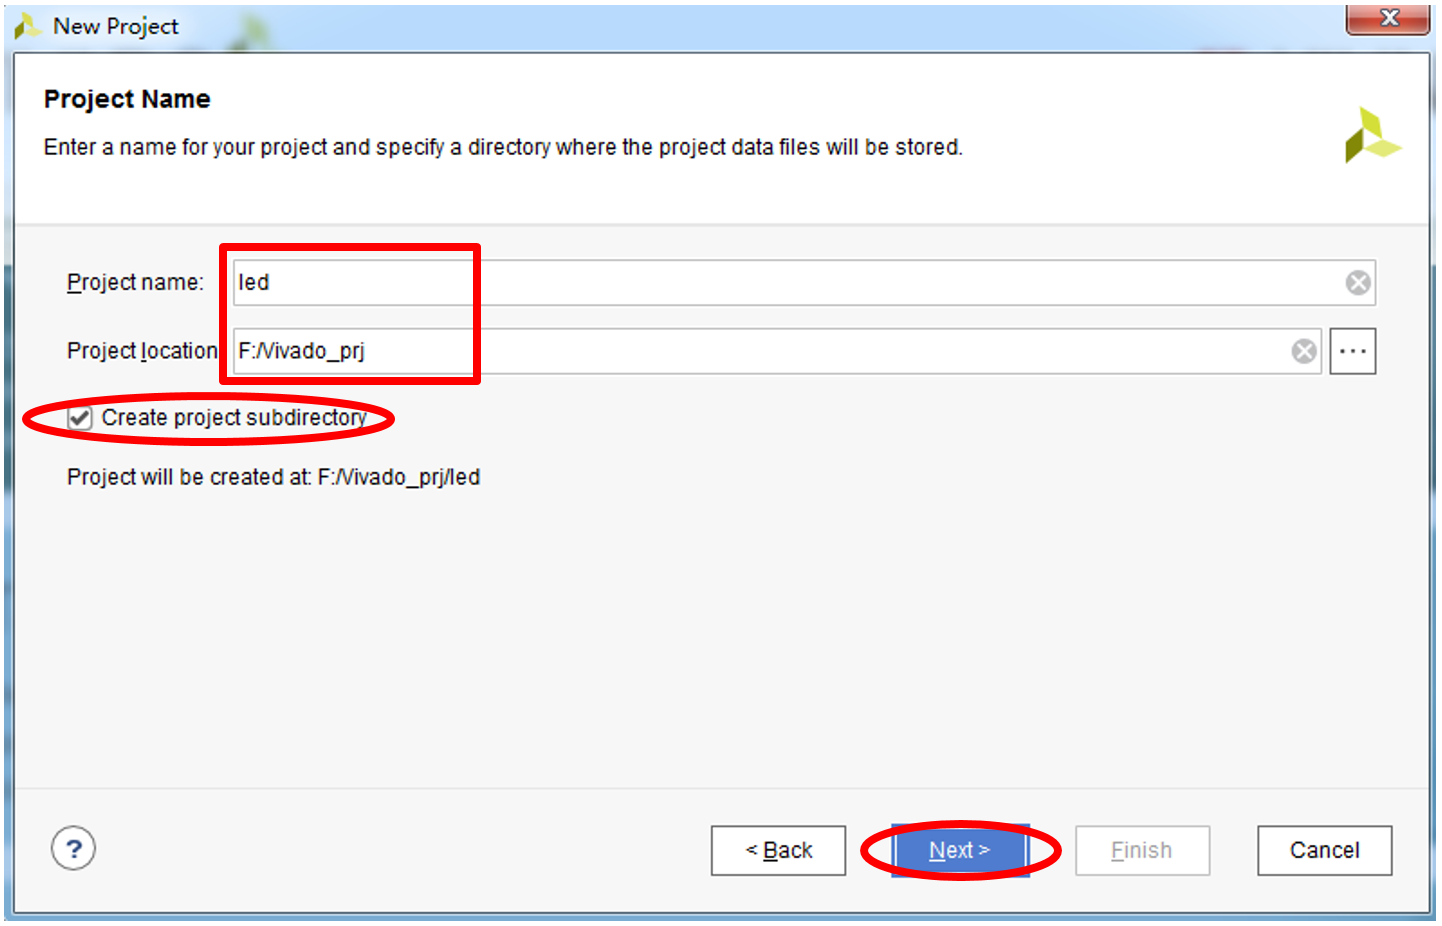
\includegraphics[width=1.0\linewidth]{assets/08/vivado_set_project_name.png}
  \caption{设置工程名称和位置}
  \label{fig:08-vivado-set-project-name}
\end{figure}

在图\ref{fig:08-vivado-set-project-type}所示的界面中选择``RTL Project''，并勾选``Do not specify sources at this time''（勾选该选项是为了跳过在新建工程的过程中添加设计源文件，如果要在新建工程时添加源文件则不勾选这个选项）。点击``Next''。

\begin{figure}[htbp]
  \centering
  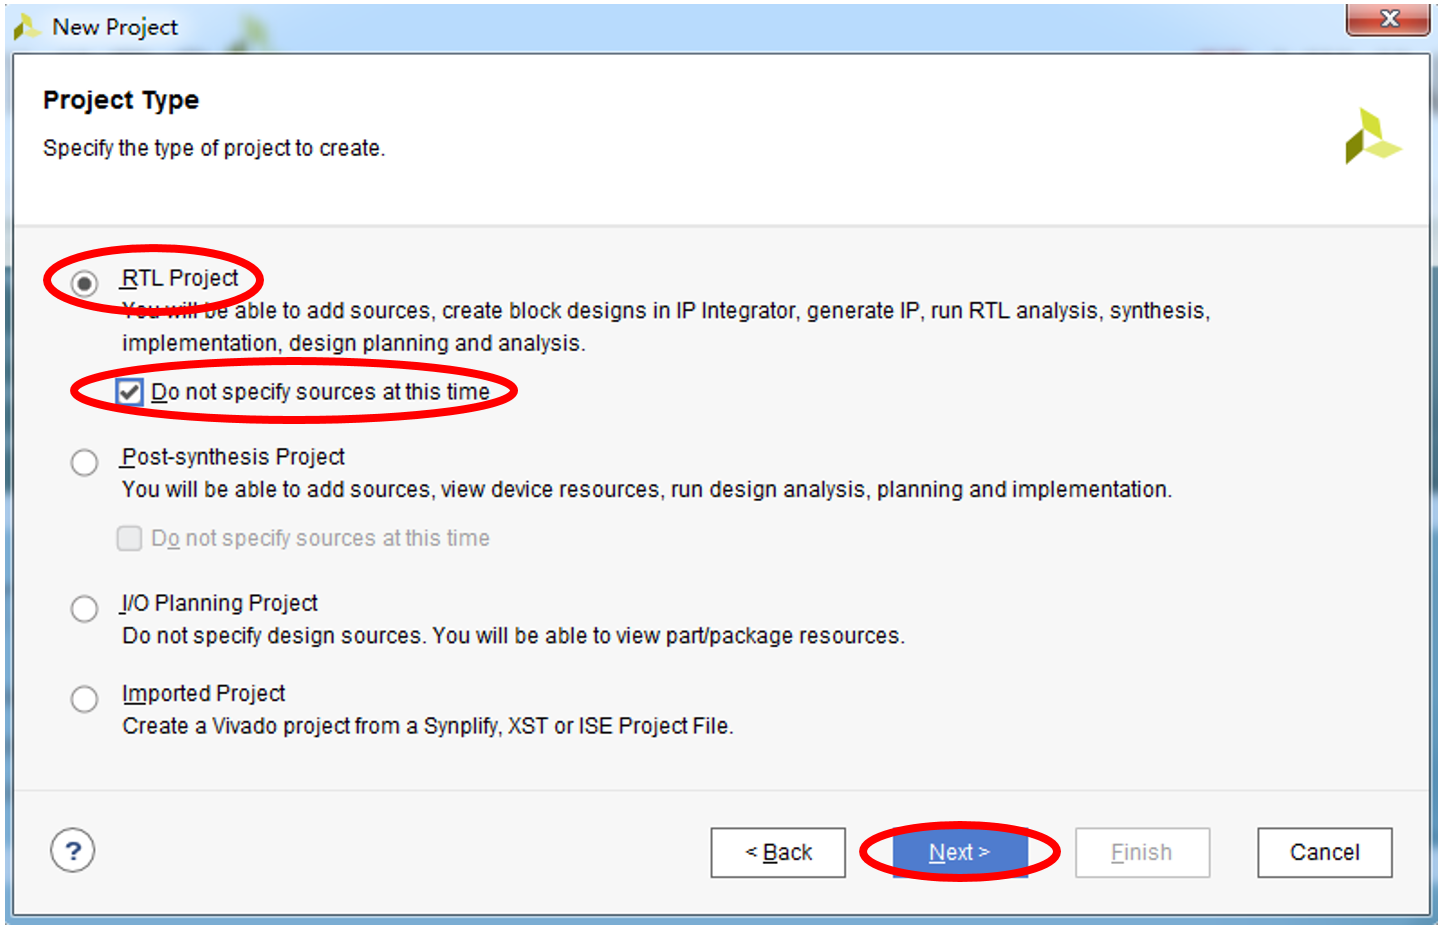
\includegraphics[width=1.0\linewidth]{assets/08/vivado_set_project_type.png}
  \caption{设置工程类型}
  \label{fig:08-vivado-set-project-type}
\end{figure}

在图\ref{fig:08-vivado-select-fpga-info} 所示的界面中选择对应的FPGA目标器件。本书推荐的本地实验箱和远程实验平台的FPGA型号一样。在``Family''中选择``Artix 7''，在``Package''中选择``fbg676''，在筛选得到的型号里面选择``xc7a200tfbg676-1''。上述选择完毕后点击``Next''。

\begin{figure}[htbp]
  \centering
  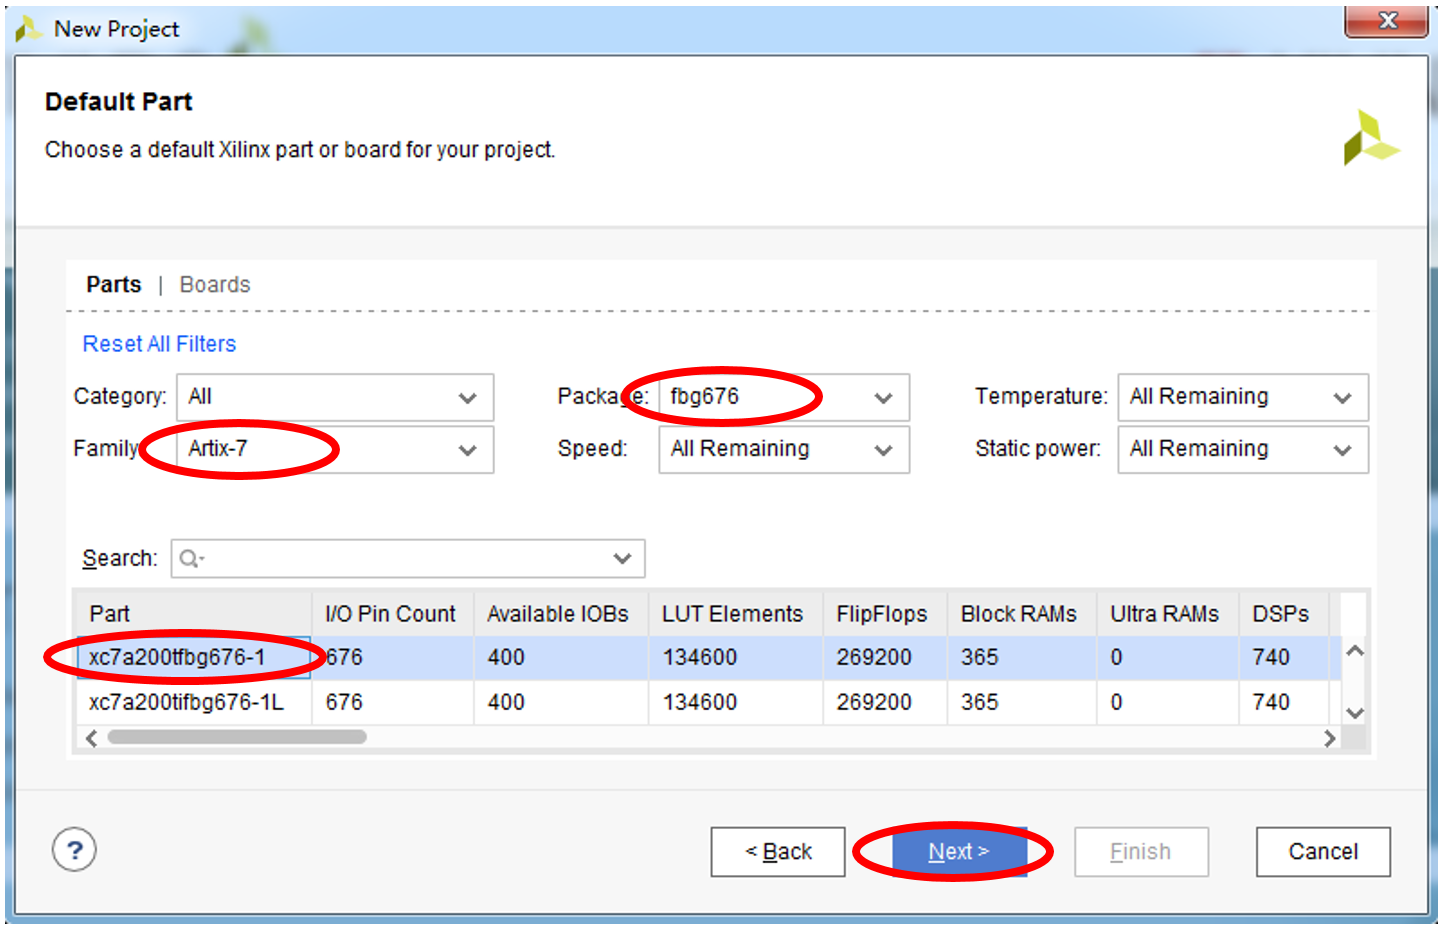
\includegraphics[width=1.0\linewidth]{assets/08/vivado_select_fpga_info.png}
  \caption{选择目标器件}
  \label{fig:08-vivado-select-fpga-info}
\end{figure}

在图\ref{fig:08-vivado-project-info-confirm} 所示的界面中确认工程的设置信息是否正确。如果正确，则点击`` Finish''；如果不正确，则点击``上一步''，返回相应步骤进行修改。

\begin{figure}[htbp]
  \centering
  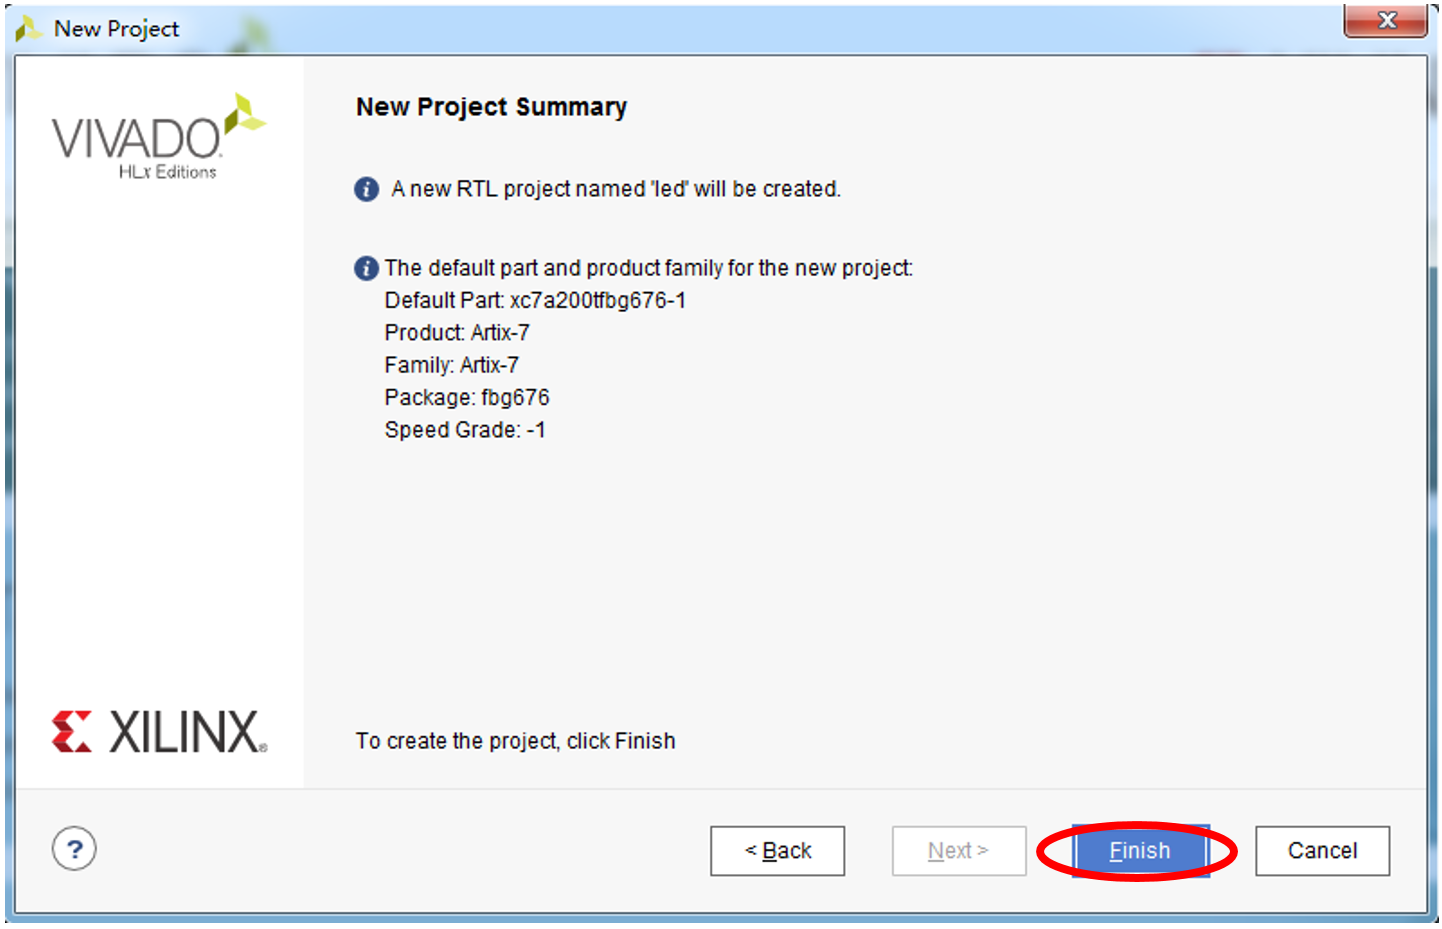
\includegraphics[width=1.0\linewidth]{assets/08/vivado_project_info_confirm.png}
  \caption{工程信息}
  \label{fig:08-vivado-project-info-confirm}
\end{figure}

完成工程新建后的界面如图\ref{fig:08-vivado-new-project-end}所示。

\begin{figure}[htbp]
  \centering
  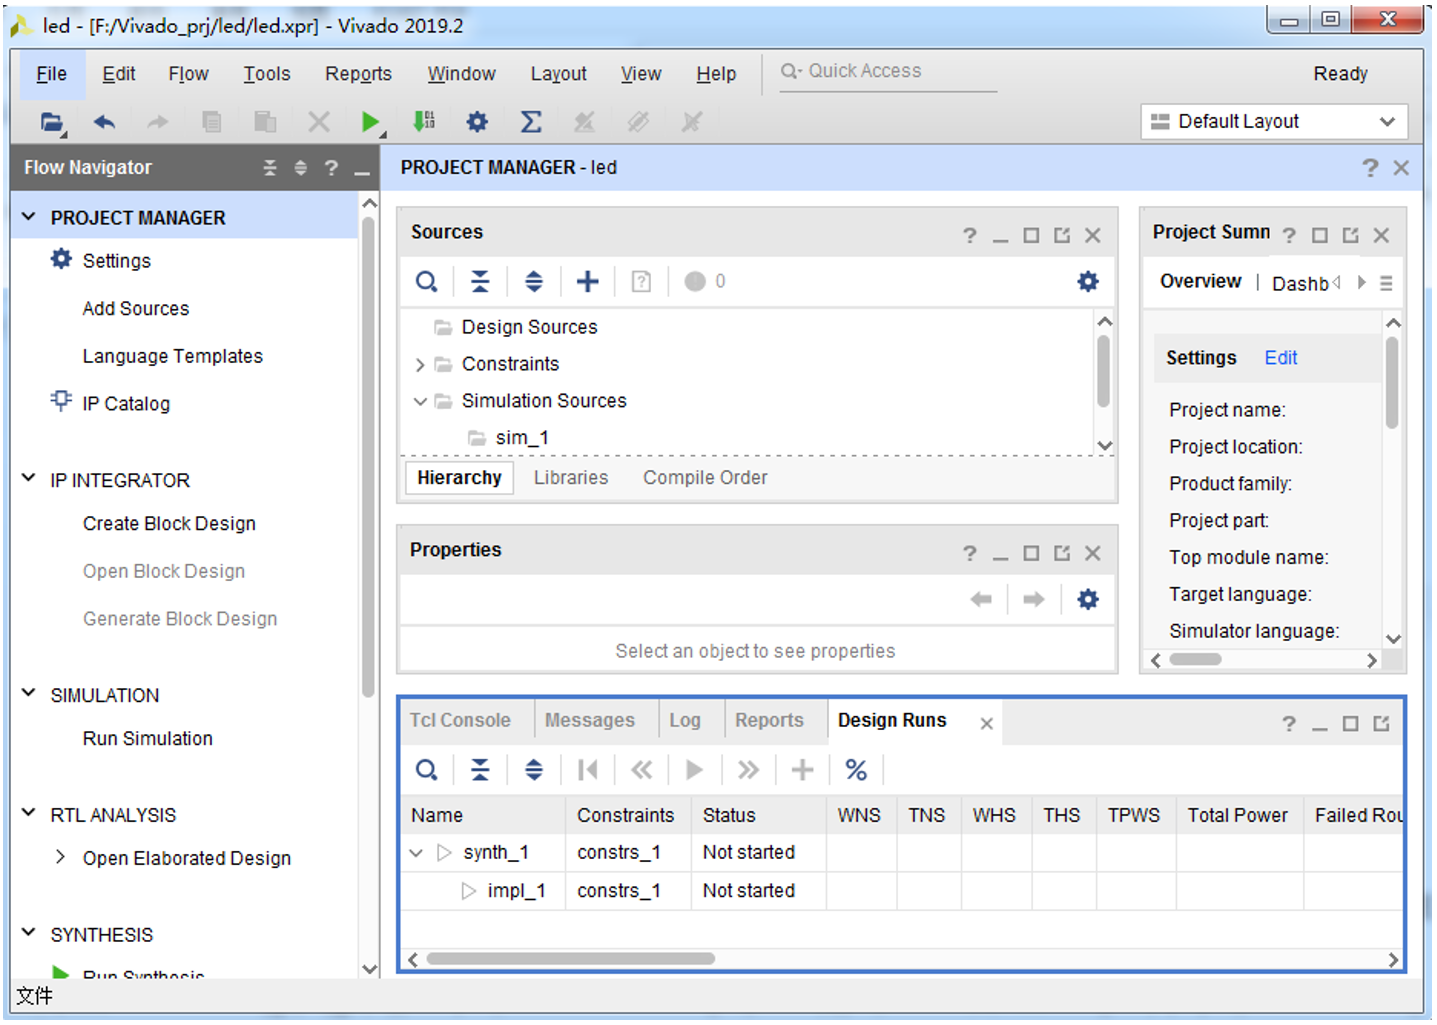
\includegraphics[width=1.0\linewidth]{assets/08/vivado_new_project_end.png}
  \caption{新建工程完成的界面}
  \label{fig:08-vivado-new-project-end}
\end{figure}

\subsection{添加设计文件}\label{sec:08-verification-and-implementation-005}

我们以使用Verilog完成RTL设计为例来说明如何添加设计文件。Verilog代码都是以``.v''为后缀名的文件，可以先在其他文件编辑器里写好代码，再添加到新建的工程中，也可以在工程中新建一个文件再编辑它。

首先添加源文件。在``Flow Navigator''窗口下的``PROJECT MANAGER''下点击``Add sources''，或者点击``Sources''窗口下``Add Sources''按钮（参见图\ref{fig:08-vivado-add-source-file}），也可以使用快捷键``Alt + A''添加源文件。

\begin{figure}[htbp]
  \centering
  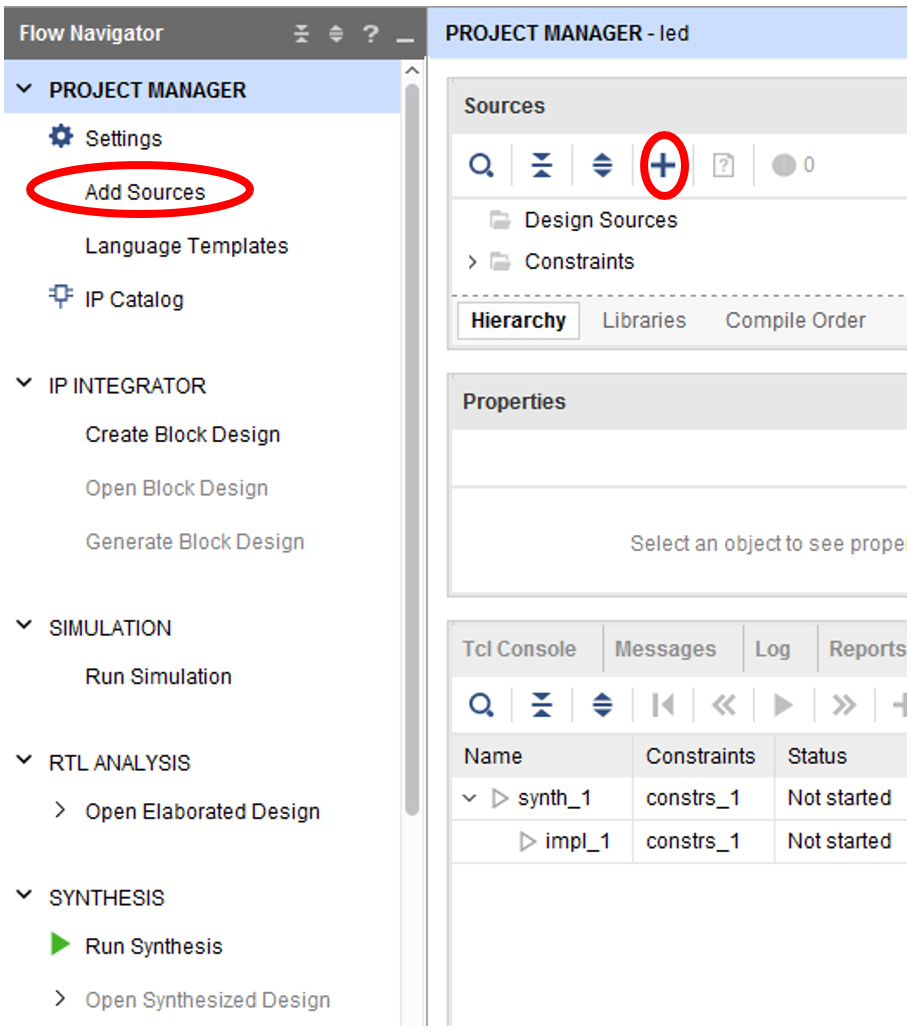
\includegraphics[width=1.0\linewidth]{assets/08/vivado_add_source_file.png}
  \caption{添加源文件}
  \label{fig:08-vivado-add-source-file}
\end{figure}

然后添加设计文件。选择``Add or create design sources''来添加或新建Verilog/VHDL源文件，再点击``Next''，如图\ref{fig:08-vivado-add-sources-next}所示。

\begin{figure}[htbp]
  \centering
  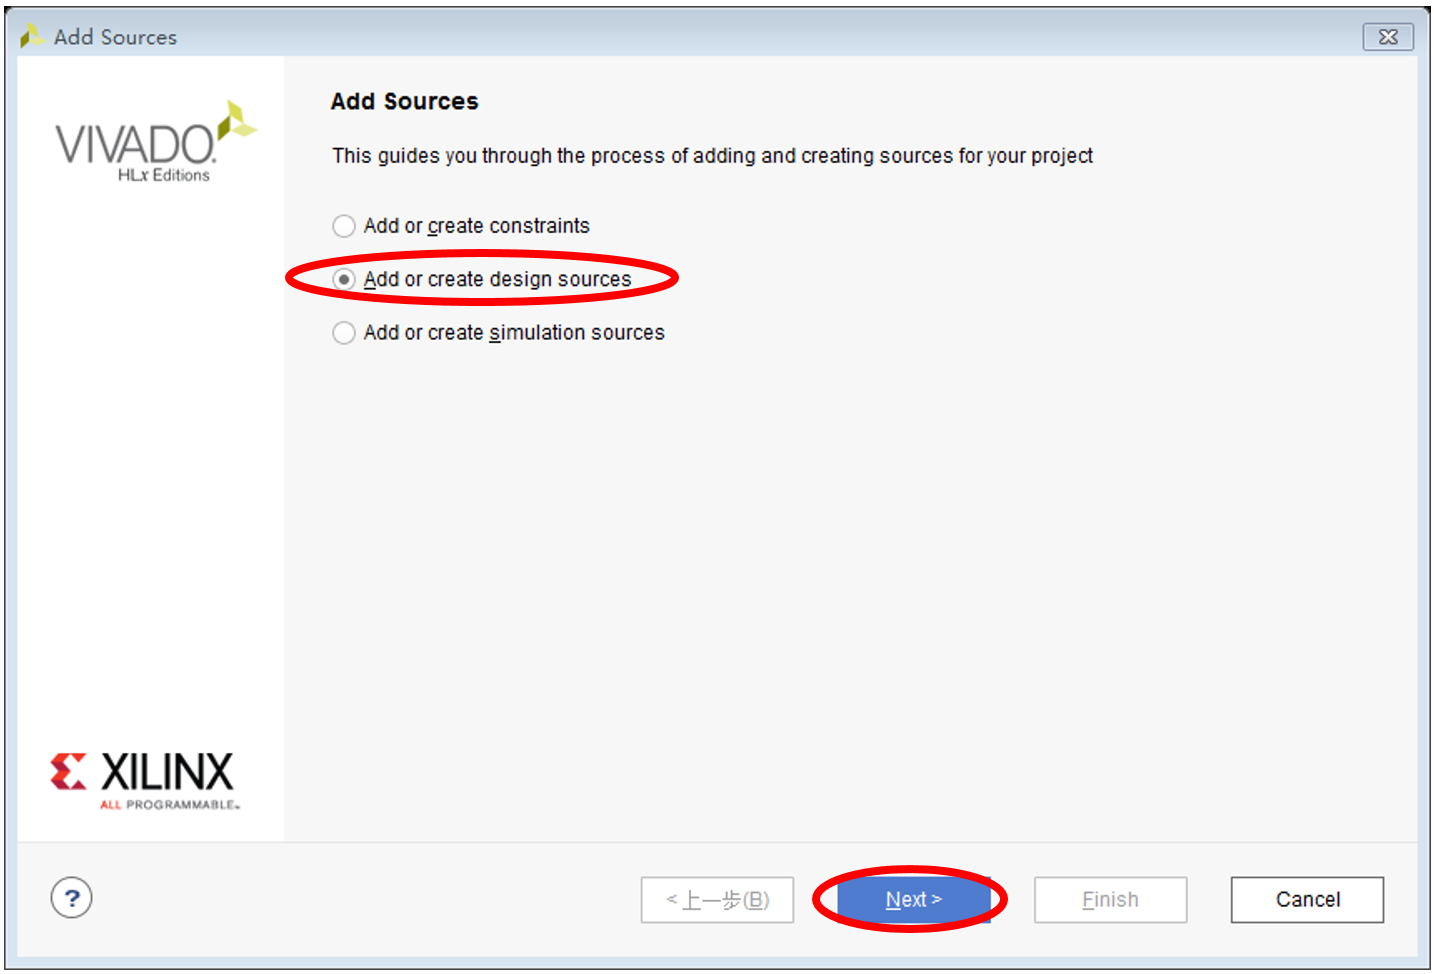
\includegraphics[width=1.0\linewidth]{assets/08/vivado_add_sources_next.png}
  \caption{添加设计文件}
  \label{fig:08-vivado-add-sources-next}
\end{figure}

接下来添加或者新建设计文件。如添加已有设计文件或者添加包含已有设计文件的文件夹，可以选择``Add Files''或者``Add Directories''，如图 所示，然后在文件浏览窗口选择已有的设计文件完成添加。

\begin{figure}[htbp]
  \centering
  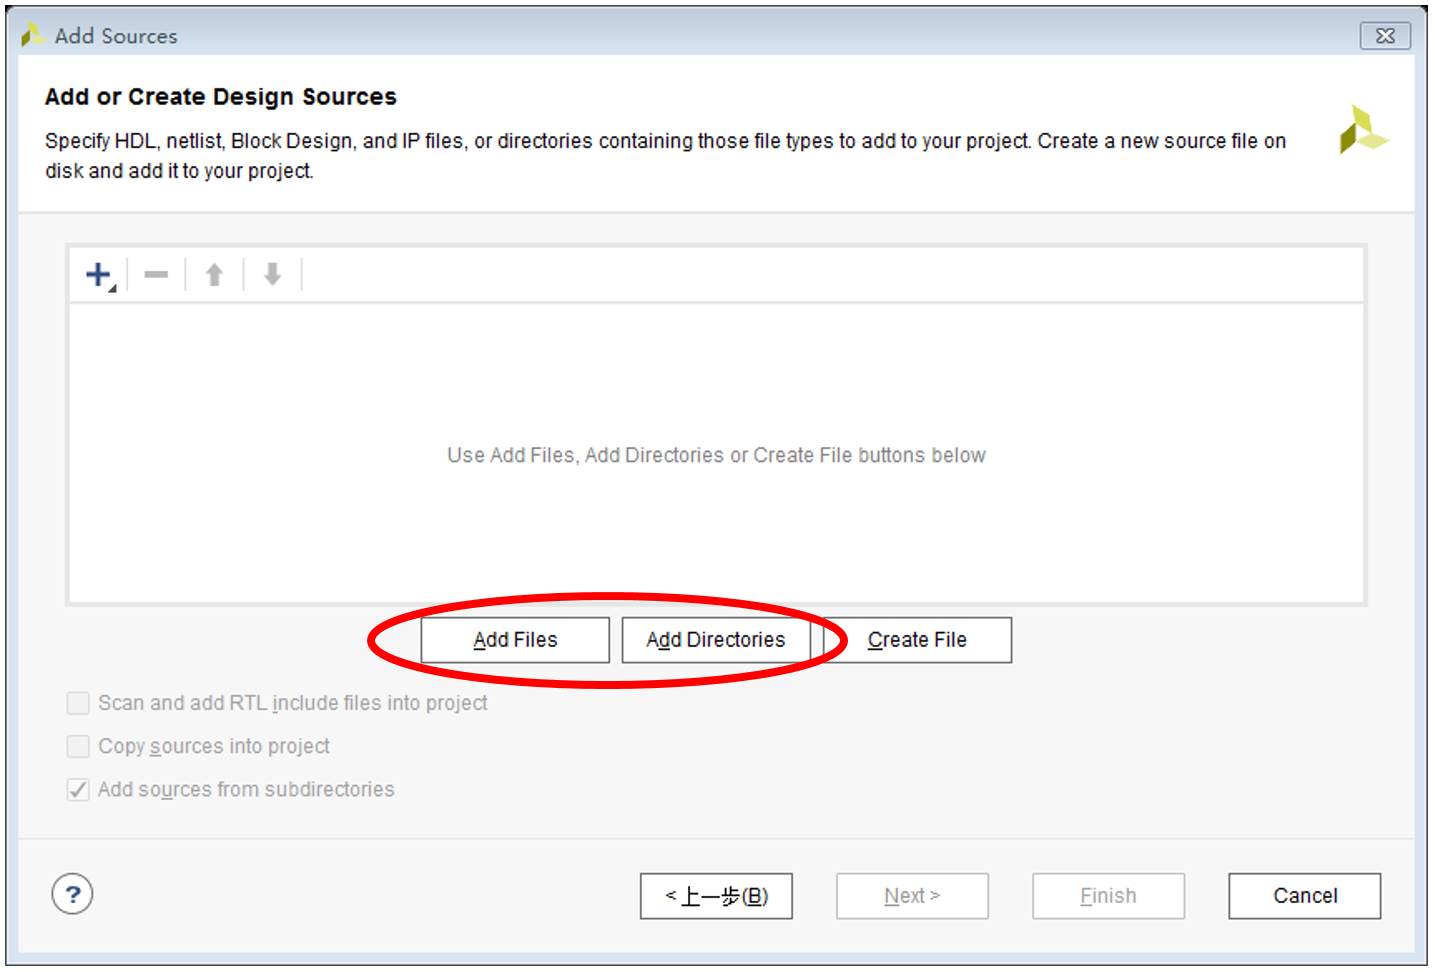
\includegraphics[width=1.0\linewidth]{assets/08/vivado_add_existing_files.png}
  \caption{添加已有设计文件}
  \label{fig:08-vivado-add-existing-files}
\end{figure}

\subsection{添加约束文件}\label{sec:08-verification-and-implementation-006}

添加约束文件有两种方法，一种是利用Vivado中I/O Planning功能，另一种是直接创建XDC约束文件，手动输入约束命令后再添加加工程中。这里主要介绍第二种方法。

首先点击``Add Sources''，选择``Add or create constraints''，点击``Next''，如图

\begin{figure}[htbp]
  \centering
  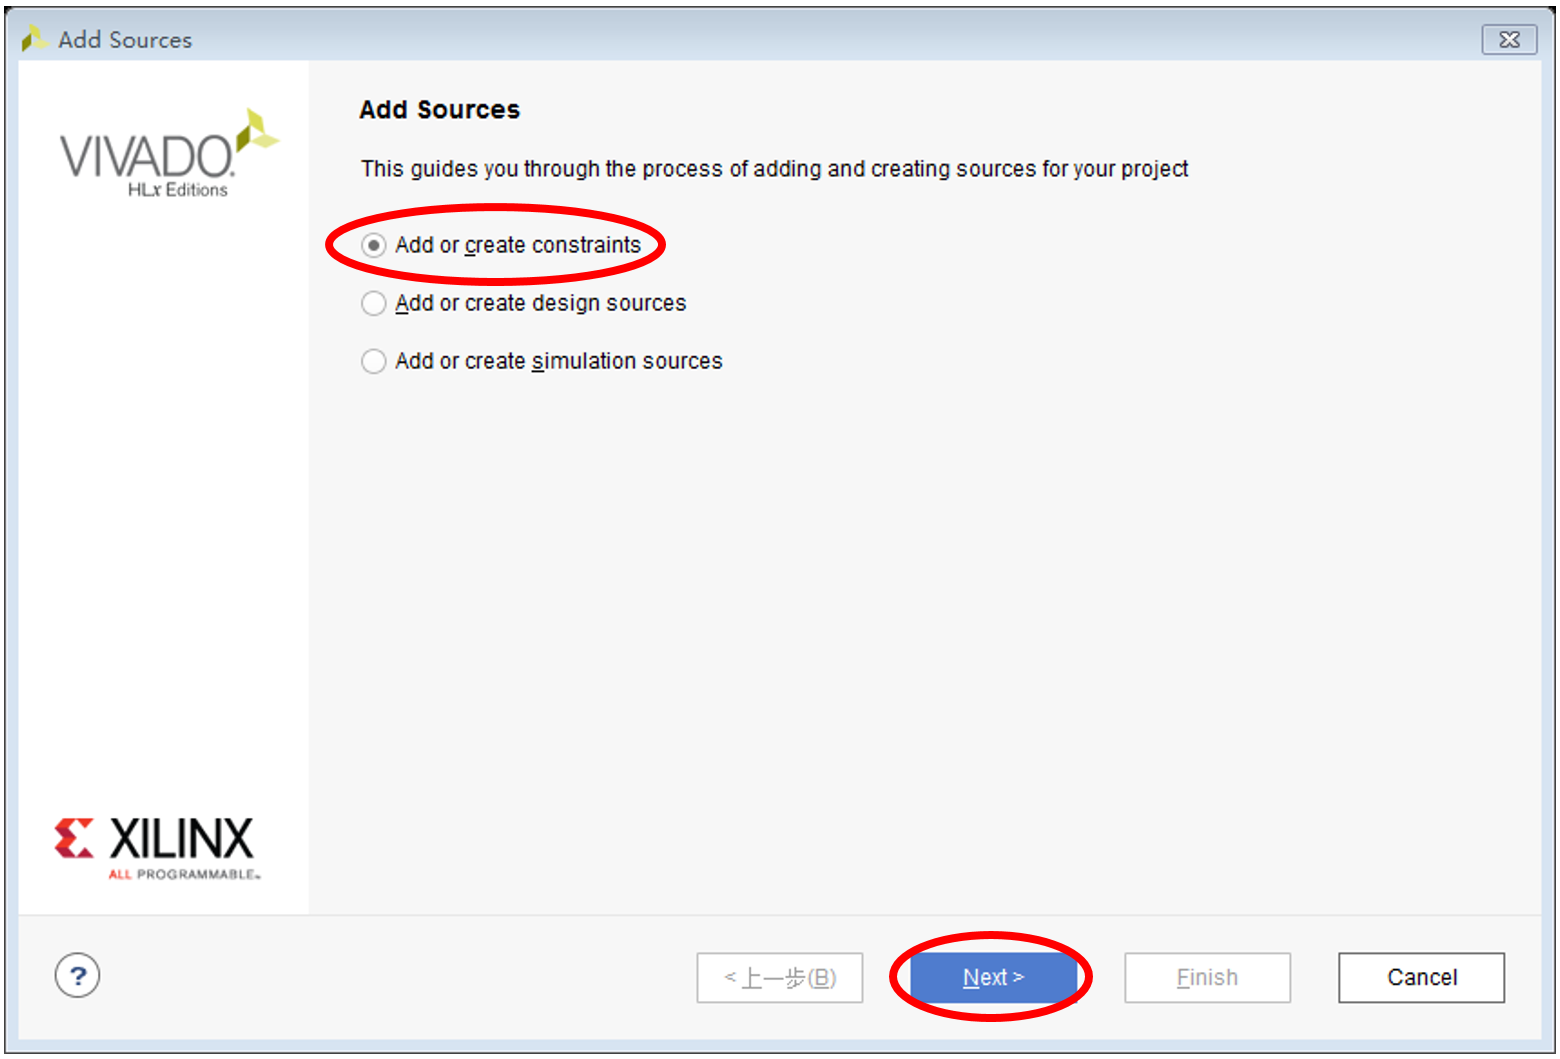
\includegraphics[width=1.0\linewidth]{assets/08/vivado_add_constraints_sources.png}
  \caption{添加约束}
  \label{fig:08-vivado-add-constraints-sources}
\end{figure}

然后添加或创建约束文件。如果采用添加已经编辑好的约束文件的方式，则如图\ref{fig:08-vivado-add-constraints-files}所示，点击``Add Files''。

\begin{figure}[htbp]
  \centering
  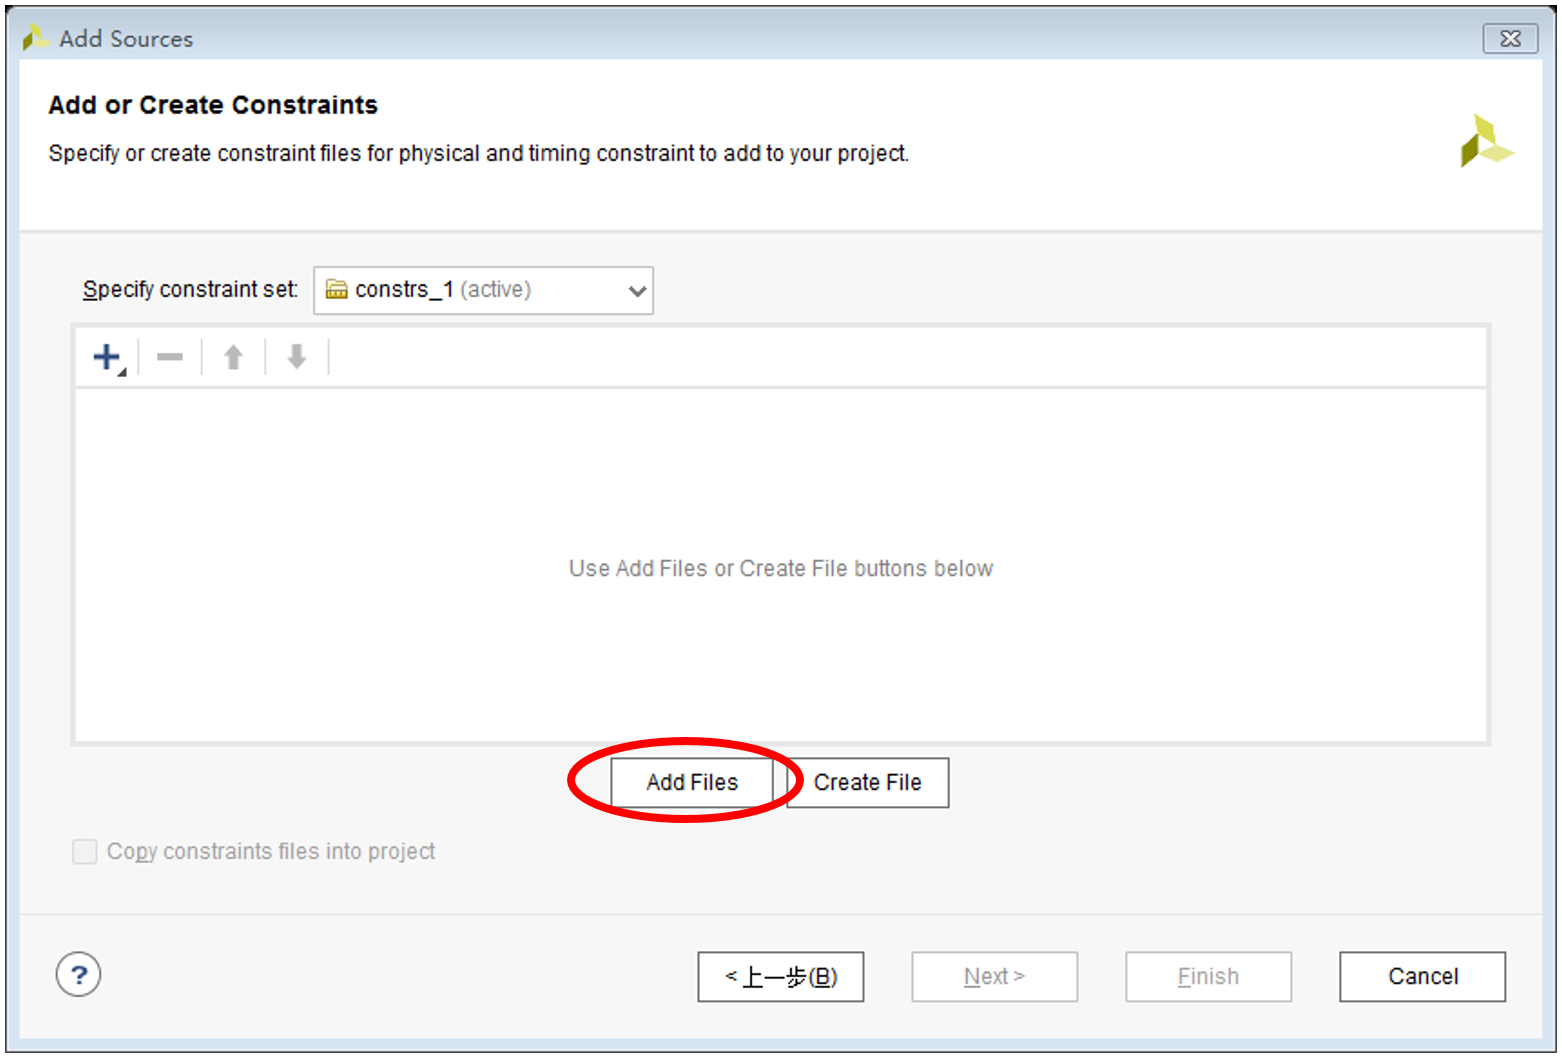
\includegraphics[width=1.0\linewidth]{assets/08/vivado_add_constraints_files.png}
  \caption{添加约束文件}
  \label{fig:08-vivado-add-constraints-files}
\end{figure}

\textbf{Note:} MegaSoC中百芯开发板的IO管脚和时序约束主要位于\url{https://github.com/BUAA-CI-LAB/MegaSoC/blob/master/Board/BaiXin/io.xdc}文件中

\subsection{综合实现和生成比特流文件}\label{sec:08-verification-and-implementation-007}

在``Flow Navigator''中点击``PROGRAM AND DEBUG''下的``Generate Bitstream''选项，工程会自动完成综合、布局布线、比特流文件生成的工作。如图\ref{fig:08-vivado-generate-bitstream}所示。完成之后，可点击``Open Implemented Design''来查看工程实现结果。

\begin{figure}[htbp]
  \centering
  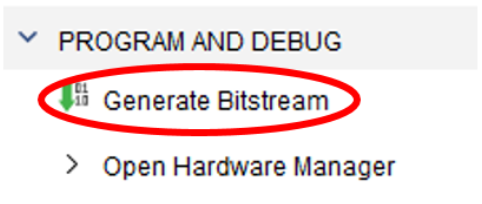
\includegraphics[width=1.0\linewidth]{assets/08/vivado_generate_bitstream.png}
  \caption{生成比特流文件}
  \label{fig:08-vivado-generate-bitstream}
\end{figure}

如果出现图\ref{fig:08-vivado-indicate-resynthesis}所示的提示，意味着综合过期，需重新运行综合和实现。这时点击``Yes''，在弹出的``Launch Runs''窗口点击``OK''。

\begin{figure}[htbp]
  \centering
  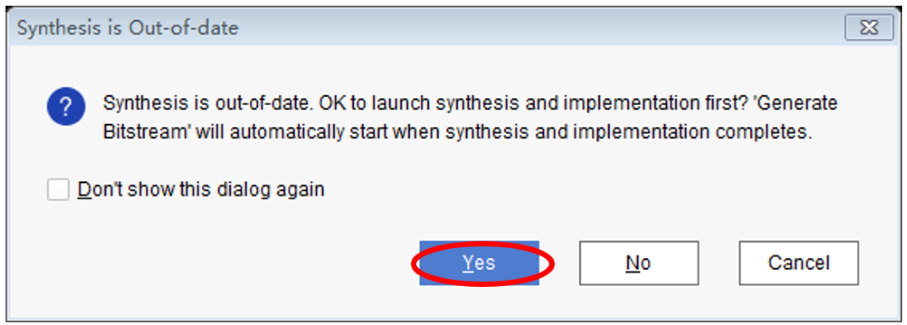
\includegraphics[width=1.0\linewidth]{assets/08/vivado_indicate_resynthesis.png}
  \caption{提示重新运行综合和实现}
  \label{fig:08-vivado-indicate-resynthesis}
\end{figure}

\subsection{烧写比特流文件}\label{sec:08-verification-and-implementation-008}

如果选用的是本地FPGA实验平台，那么在比特流文件生成后就可以进入烧写配置FPGA的阶段了。具体操作是：在比特流文件生成完成的窗口选择``Open Hardware Manager''，点击OK，进入硬件管理界面，如图\ref{fig:08-vivado-open-hardware-manager}所示。连接FPGA开发板的电源线和与电脑的下载线，打开FPGA电源。

\begin{figure}[htbp]
  \centering
  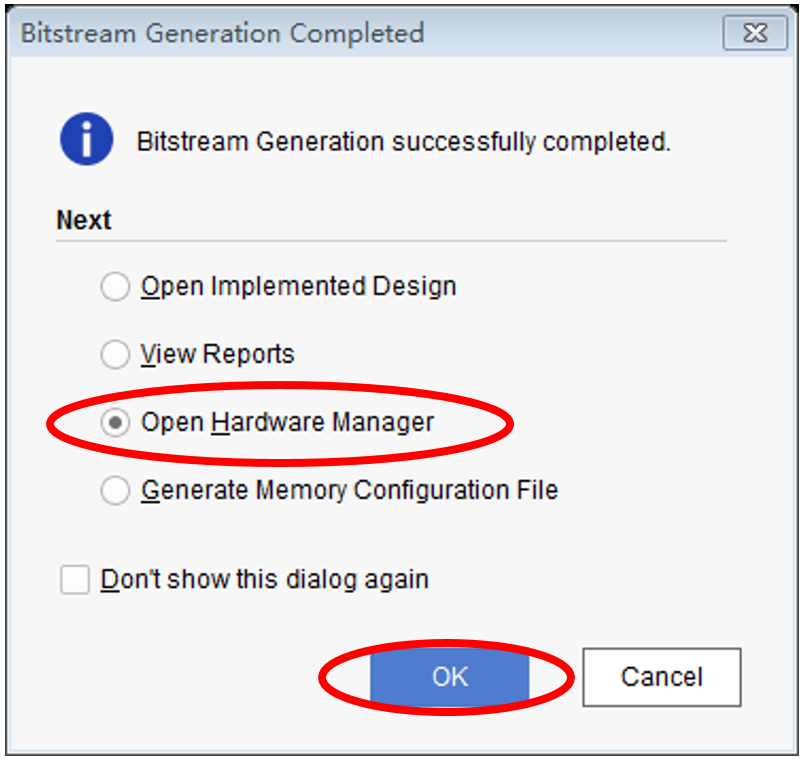
\includegraphics[width=1.0\linewidth]{assets/08/vivado_open_hardware_manager.png}
  \caption{打开硬件管理器}
  \label{fig:08-vivado-open-hardware-manager}
\end{figure}

在``Hardware Manager''窗口的提示信息中，点击``Open target''下拉菜单的``Open New Target''（或在``Flow Navigator'' 下 的``PROGRAM AND DEBUG'' 中展开``Open Hardware Manager''， 点击``Open Target Open New Target''），也可以选择``AutoConnect''来自动连接器件，如图\ref{fig:08-vivado-open-new-target}所示。一般的我们选择``AutoConnect''

\begin{figure}[htbp]
  \centering
  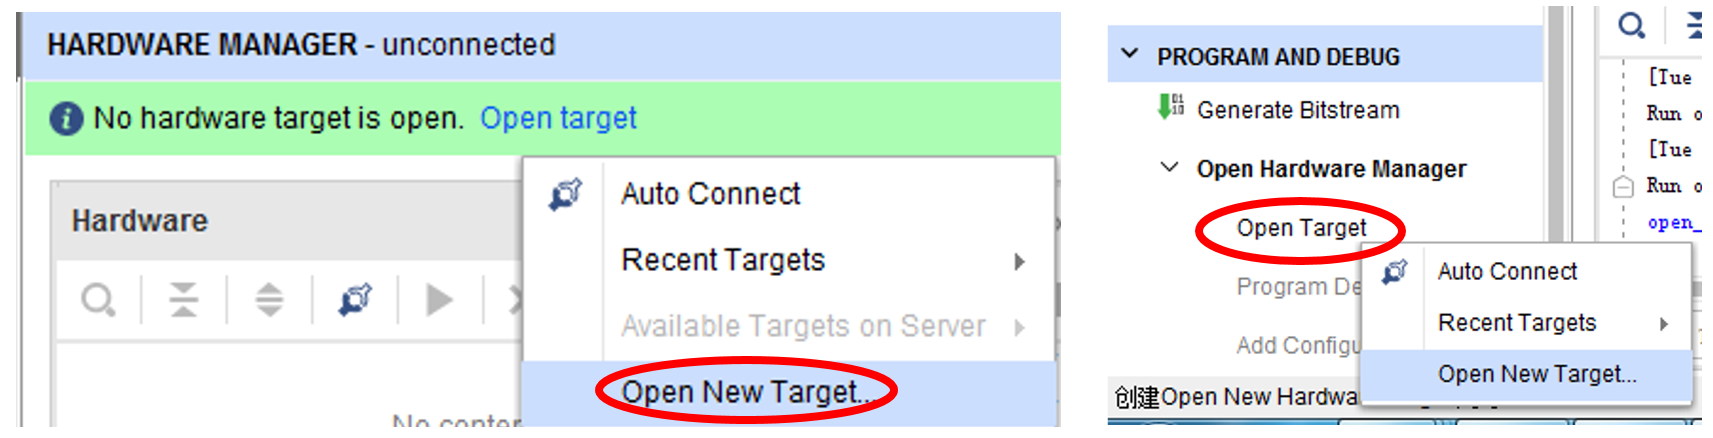
\includegraphics[width=1.0\linewidth]{assets/08/vivado_open_new_target.png}
  \caption{打开新目标}
  \label{fig:08-vivado-open-new-target}
\end{figure}

接下来对目标硬件编程。在``Hardware''窗口右键单击目标器件``xc7a200t\_0''，选择``Program Device\ldots''；或者在``Flow Navigator''窗口中点击``PROGRAM AND DEBUG Hardware Manager Program Device''。如图\ref{fig:08-vivado-program-device}所示。

\begin{figure}[htbp]
  \centering
  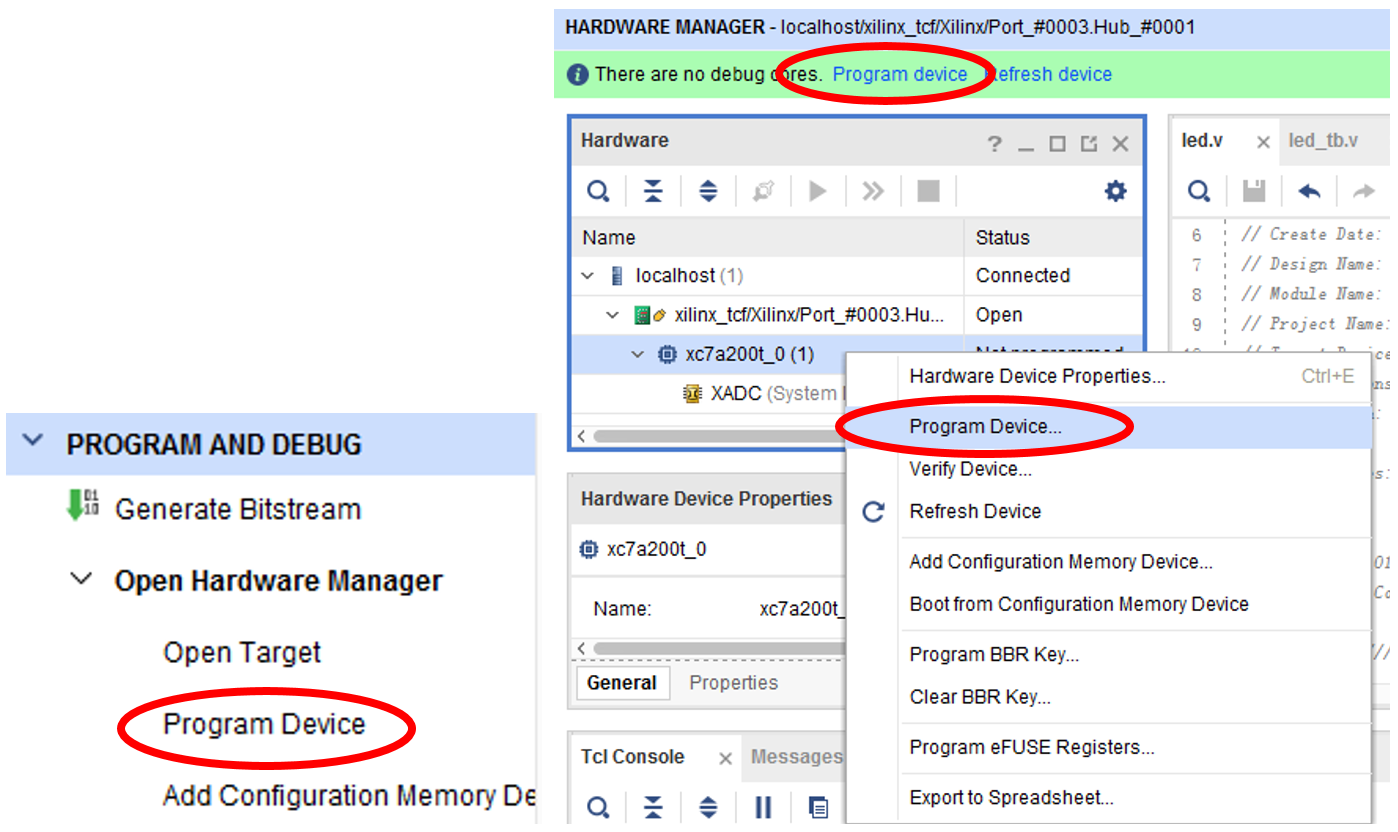
\includegraphics[width=1.0\linewidth]{assets/08/vivado_program_device.png}
  \caption{目标硬件编程}
  \label{fig:08-vivado-program-device}
\end{figure}

选择下载的比特流文件，点击``Program''。完成下载后，``Hardware''窗口下的``xc7a200t\_0''的状态变成``Programmed''，如图\ref{fig:08-vivado-fpga-programmed}所示。

\begin{figure}[htbp]
  \centering
  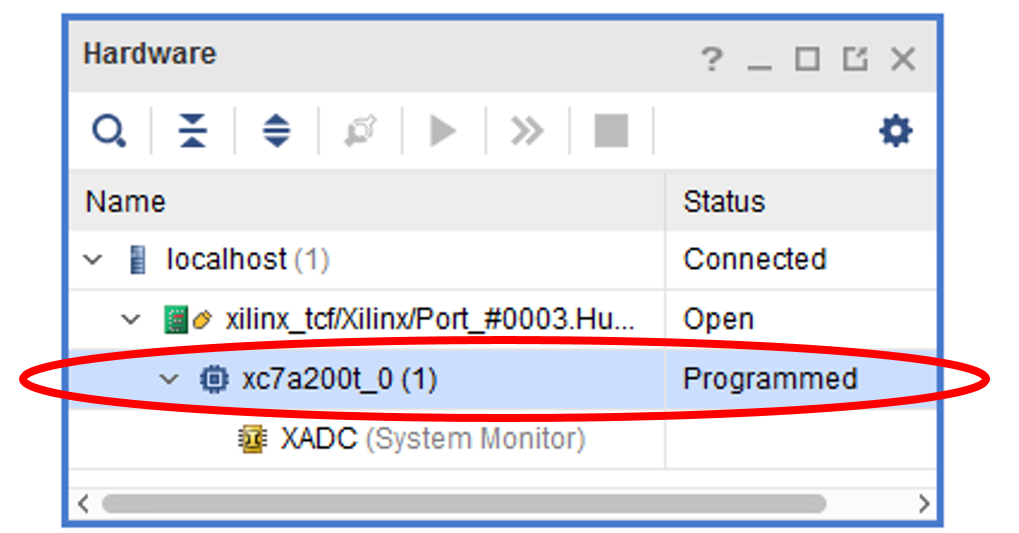
\includegraphics[width=1.0\linewidth]{assets/08/vivado_fpga_programmed.png}
  \caption{FPGA 编程完成}
  \label{fig:08-vivado-fpga-programmed}
\end{figure}

连接串口后即可看到SoC输出，如图\ref{fig:08-vivado-fpga-output}所示。在Linux系统下，可以使用各种软件来进行串口通信、音视频播放、USB连接等功能的测试。

\begin{figure}[htbp]
  \centering
  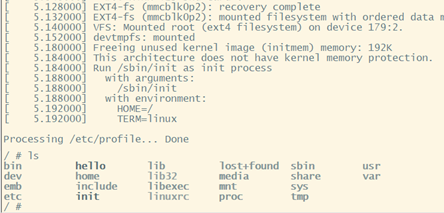
\includegraphics[width=1.0\linewidth]{assets/08/vivado_fpga_output.png}
  \caption{串口输出}
  \label{fig:08-vivado-fpga-output}
\end{figure}

\section{芯片实现的前端设计}\label{sec:08-verification-and-implementation-009}

芯片的整体实现流程如图\ref{fig:08-chip-flow}所示。

\begin{figure}[htbp]
  \centering
  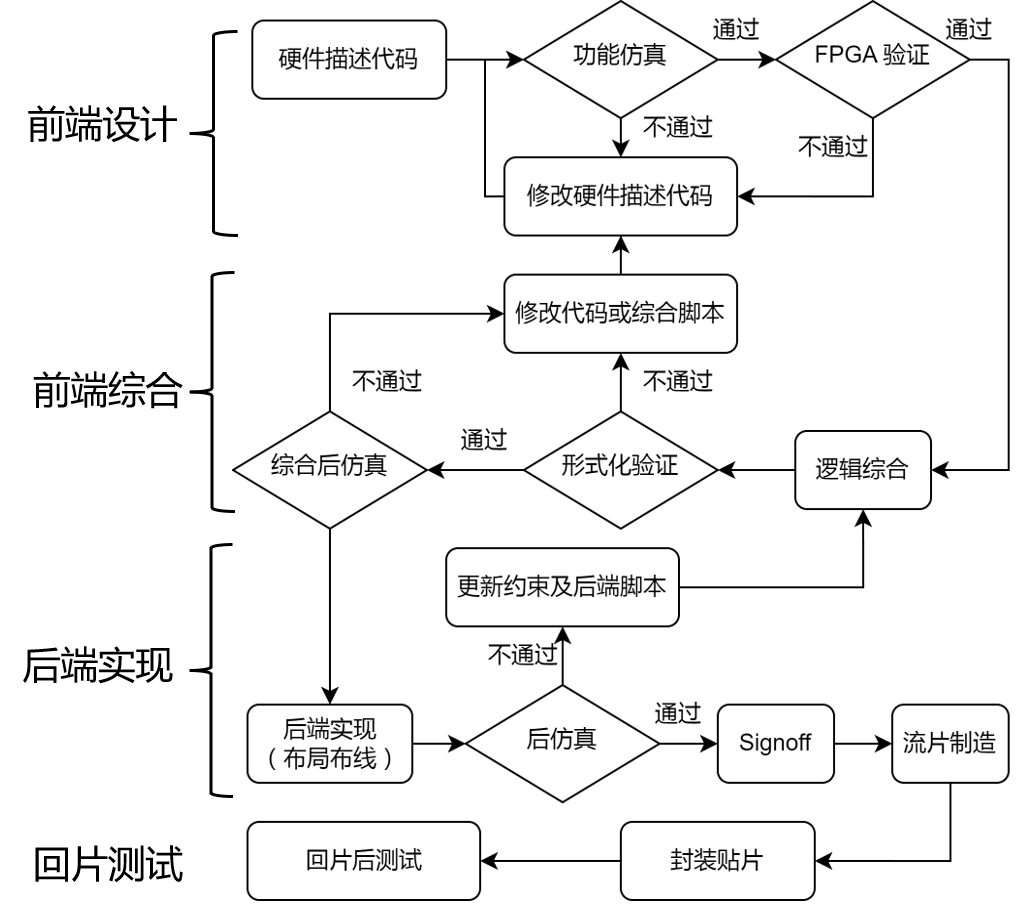
\includegraphics[width=0.7\linewidth]{assets/08/芯片设计流程.png}
  \caption{芯片设计流程}
  \label{fig:08-chip-flow}
\end{figure}

其中设计部分包括两款CPU以及一款SOC（两款CPU芯片都采用一款SOC），EULA CPU核心设计参考第3章内容，LAIN CPU核心设计参考第4章，SOC设计参考第7章。

\section{芯片实现的测试与验证}\label{sec:08-verification-and-implementation-010}

RTL代码的仿真测试在第6章敏捷开发流程中已经详细介绍，包括使用verilator仿真、Difftest差分测试CPU核心、以及针对SOC的接口与外设验证等；FPGA仿真测试在8.3中已经详细描述。本部分主要介绍一下一致性验证以及针对综合后网表仿真的过程。

\subsection{一致性验证}\label{sec:08-verification-and-implementation-011}

一般使用Synopsys formality来进行一致性验证。一致性验证主要是验证RTL代码与综合后的门级网表之间的逻辑等价性（与时序无关）。实际上除了上述情况外，还有将综合网表与布局布线后网表进行比较的情况。一般设计形式发生变化就需要做一致性验证。

formality工具可以使用GUI用户界面进行操作，也可以使用tcl脚本文件。下面以脚本文件为例来说明formality工具的使用过程：

首先初始化synopsys formality脚本，并使用\emph{fm\_shell}命令运行formality。

% 代码语言：BookShell
\begin{CodeBlock}[language=BookShell]
source /path/to/synopsys_setup.bash
fm_shell -file fm_check.tcl
#fm -gui -file fm_check.tcl 使用gui界面运算脚本
\end{CodeBlock}

下面是fm\_check.tcl脚本包含的具体指令：

\begin{enumerate}
\def\labelenumi{\arabic{enumi}.}
\tightlist
\item
  添加.svf文件（DC综合生成的文件，包含综合时的优化记录）
\end{enumerate}

% 代码语言：BookTcl
\begin{CodeBlock}[language=BookTcl]
set_svf -append {/home/IC/soc/form_test/svf/test.svf}
\end{CodeBlock}

\begin{enumerate}
\def\labelenumi{\arabic{enumi}.}
\setcounter{enumi}{1}
\tightlist
\item
  读入rtl设计文件
\end{enumerate}

% 代码语言：BookTcl
\begin{CodeBlock}[language=BookTcl]
read_verilog -container r -libname WORK -05 { /home/IC/soc/form_test/rtl/verilog_test.v }
\end{CodeBlock}

\begin{enumerate}
\def\labelenumi{\arabic{enumi}.}
\setcounter{enumi}{2}
\tightlist
\item
  设置DC工具路径
\end{enumerate}

% 代码语言：BookTcl
\begin{CodeBlock}[language=BookTcl]
set hdlin_dwroot /opt/Synopsys/DC2015
\end{CodeBlock}

\begin{enumerate}
\def\labelenumi{\arabic{enumi}.}
\setcounter{enumi}{3}
\tightlist
\item
  读取综合时使用的db库文件
\end{enumerate}

% 代码语言：BookTcl
\begin{CodeBlock}[language=BookTcl]
read_db { /home/IC/soc/form_test/db/fast.db }
\end{CodeBlock}

\begin{enumerate}
\def\labelenumi{\arabic{enumi}.}
\setcounter{enumi}{4}
\tightlist
\item
  设置顶层模块
\end{enumerate}

% 代码语言：BookTcl
\begin{CodeBlock}[language=BookTcl]
set_top r:/WORK/verilog_test
\end{CodeBlock}

\begin{enumerate}
\def\labelenumi{\arabic{enumi}.}
\setcounter{enumi}{5}
\tightlist
\item
  读入网表文件
\end{enumerate}

% 代码语言：BookTcl
\begin{CodeBlock}[language=BookTcl]
read_verilog -container i -libname WORK -05 { /home/IC/soc/form_test/netlist/netlist_test.v }
\end{CodeBlock}

\begin{enumerate}
\def\labelenumi{\arabic{enumi}.}
\setcounter{enumi}{6}
\tightlist
\item
  设置顶层模块
\end{enumerate}

% 代码语言：BookTcl
\begin{CodeBlock}[language=BookTcl]
set_top i:/WORK/netlist_test
\end{CodeBlock}

\begin{enumerate}
\def\labelenumi{\arabic{enumi}.}
\setcounter{enumi}{7}
\tightlist
\item
  验证待比较两者的IO端口等是否匹配
\end{enumerate}

% 代码语言：BookTcl
\begin{CodeBlock}[language=BookTcl]
match
\end{CodeBlock}

\begin{enumerate}
\def\labelenumi{\arabic{enumi}.}
\setcounter{enumi}{8}
\tightlist
\item
  验证RTL和网表的逻辑功能是否相同
\end{enumerate}

% 代码语言：BookTcl
\begin{CodeBlock}[language=BookTcl]
verify
\end{CodeBlock}

\subsection{综合后仿真（网表仿真）}\label{sec:08-verification-and-implementation-012}

综合后的网表延时包含了标准单元的延时，此时电路具有了时序信息。网表仿真的过程实际上与RTL代码仿真没有太大的区别，只是将RTL代码替换为生成的网表文件进行仿真，此时仿真包含了时序信息。下面给出使用VCS工具仿真的过程：

预处理及链接.sdf文件（包含标准单元延时的文件）：

% 代码语言：BookShell
\begin{CodeBlock}[language=BookShell]
# 删除上一次链接的文件
rm -f test.sdf
# 链接sdf文件
ln -s /path/to/test.sdf
# 执行make
make test
\end{CodeBlock}

同目录下的Makefile，其中netlist.f是包含生成的网表文件、库文件仿真模型、测试tb的路径：

% 代码语言：BookMake
\begin{CodeBlock}[language=BookMake]
# 定义VCS编译和链接时使用的通用选项  
VCS_OPTIONS=-full64 +alwaystrigger -PP +define+VCS -debug_all +vcs+vcdpluson  
# 注意：虽然定义了VCS_OPTIONS，但在下面的test目标中并未直接使用它  
  
# 定义VCS链接时使用的特定选项  
VCS_LINK_OPTIONS=-full64 +alwaystrigger --debug_access+nomemcbk+dmptf -debug_region+cell 
-debug_all +vcs+vcdpluson +lint=TFIPC-L  
  
# 定义NOVAS PLI库的位置和相关的编译选项  
NOVAS_PLI=$(NOVAS_HOME)/share/PLI/VCS/linux64  
NOVAS_FLAGS=-P $(NOVAS_PLI)/novas.tab $(NOVAS_PLI)/pli.a  
  
# 以下是Makefile的目标部分  
  
# test目标：用于编译和仿真test设计  
test:  
    # 使用vcs命令进行编译和链接  
    # -sverilog 启用SystemVerilog支持  
    # -sdf typ:test:test.sdf 指定SDF文件用于时序仿真  
    # +v2k 用于向后兼容Verilog-2001，非必须 
    # +define+FOR_SIM=1 定义宏FOR_SIM，值为1  
    # +neg_tchk 用于检查负时间延迟或类似问题的选项  
    # $(VCS_LINK_OPTIONS) 使用前面定义的VCS链接选项  
    # -o bin/$@ 指定输出可执行文件的名称，$@是Makefile的自动变量，代表目标名（test）  
    # -f netlist.f 指定包含Verilog源文件列表的文件  
    # -debug_pp 用于调试的特定选项，具体含义依赖于VCS版本  
    # $(NOVAS_FLAGS) 使用前面定义的NOVAS PLI相关选项  
    vcs -sverilog -sdf typ:test:test.sdf +v2k +define+FOR_SIM=1 +neg_tchk 
    $(VCS_LINK_OPTIONS) -o bin/$@ -f netlist.f -debug_pp $(NOVAS_FLAGS)
      
    # 执行仿真，并将输出重定向到日志文件，同时显示时间  
    # bin/$@ 执行前面编译生成的可执行文件
    # +vpdfile+bin/$@.vpd 生成VPD文件用于调试  
    # tee命令用于同时输出到终端和文件  
    time bin/$@ +vpdfile+bin/$@.vpd | tee bin/$@.log  
  
# clean目标：用于清理仿真过程中生成的文件和目录  
clean :  
    # 删除csrc目录、AN.DB文件和bin目录下的所有内容  
    rm -rf csrc AN.DB  bin/*
\end{CodeBlock}

\section{芯片实现的后端设计}\label{sec:08-verification-and-implementation-013}

后端设计的流程如图\ref{fig:08-pd-flow}所示，即基于网表完成物理后端设计与实现，并探索设计流程、功耗、性能与面积上的优化。

\begin{figure}[htbp]
  \centering
  
\includegraphics[width=0.7\linewidth]{assets/08/芯片后端流程.png}
  \caption{芯片后端流程}
  \label{fig:08-pd-flow}
\end{figure}

本节将从这几个步骤进行一步步实践与描述。

\subsection{物理设计}\label{sec:08-verification-and-implementation-014}

物理设计包含芯片布局规划与布局、时钟树综合、布线等过程。

\subsubsection{芯片布局规划与布局}\label{sec:08-verification-and-implementation-015}

1.\textbf{设计初始化}

设计初始化是将综合生成的网表导入内存，并根据前端设计的要求进行约束。在此过程中，需要进行后端设计所需数据的读取、约束的建立和多模式多角分析（MMMC）的设置。

首先，需要读取各类设计文件，包括网表文件（Verilog File）、物理信息文件（LEF File）、时序库文件（Timing Library）、时序约束文件（Timing Constraint File）、电容查找表文件（Captable File）和寄生参数抽取文件（RC Extraction File）。本设计中涉及两个网表文件：lain\_top.v 和 eula\_top.v。物理信息文件包含工艺文件、标准单元库和宏模块信息文件，以及天线效应规则检查与修复文件。电容查找表文件使用 180nm 工艺库提供的 1P6M\_-5Ia\_1TMa1\_MIM1fF\_CMAX.captbl和 1P6M\_5Ia\_1TMa1\_MIM1fF\_CMIN.captbl 文件。寄生参数抽取文件设置了 CMAX、CMIN、RCMAX、RCMIN、TYP 五种 RC Corner。时序库文件共 30 个，本设计中使用了其中的 5 个文件，它们的 PVT 条件如表\ref{fig:08-PVT-list}所示：

\begin{figure}[htbp]
  \centering
  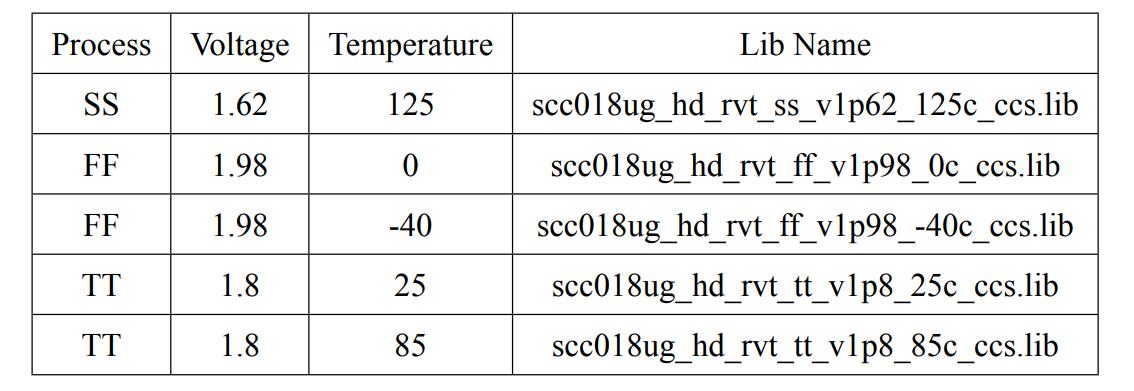
\includegraphics[width=0.7\linewidth]{assets/08/PVT_list.png}
  \caption{库文件中的PVT对照表}
  \label{fig:08-PVT-list}
\end{figure}

在多模多角分析（MMMC）时，通过 Mode、PVT Corner 和 RC Corner 组合建立View，生成 Viewdefinition 的 TCL 文件，并加载这些文件以导入多种 View。下述代码列出了本设计用到的 analysis view。包括 setup 和 hold 两种 analysis view，以及泄漏功耗和 动态功耗 analysis view：

% 代码语言：BookTcl
\begin{CodeBlock}[language=BookTcl]
set_analysis_view \
-setup [list func_ss_v1p62_125c_cmax_125 \
             func_ff_v1p98_m40c_cmin_m40 \
             func_ff_v1p98_0c_cmin_0 \
             func_ff_v1p98_m40c_cmax_m40 \
             func_ff_v1p98_0c_cmax_0 \
             func_tt_v1p8_25c_tt_25 \
             func_tt_v1p8_85c_tt_85 ] \
-hold [list func_ss_v1p62_125c_cmax_125 \
            func_ff_v1p98_m40c_cmin_m40 \
            func_ff_v1p98_0c_cmin_0 \
            func_ff_v1p98_m40c_cmax_m40 \
            func_ff_v1p98_0c_cmax_0 \
            func_tt_v1p8_25c_tt_25 \
            func_tt_v1p8_85c_tt_85 ] \
-leakage [list func_tt_v1p8_85c_tt_85] \
-dynamic [list func_tt_v1p8_85c_tt_85
\end{CodeBlock}

初始化阶段还有一些额外设置。例如，根据前端设计的要求，可以对某些区域内的标准单元设置 set\_dont\_touch 属性，防止这些单元在优化过程中被改动。此外，禁用不符合设计要求的标准单元以促进时序收敛，并将备用单元（Spare Cell）分散放置，以确保在 ECO 环节能就近找到需要的逻辑单元。以上各步骤完成了设计初始化，并确保设计在多个 analysis view 下的时序收敛和一致性。经过初始化后的设计，init\_timing 检查结果如表\ref{fig:08-timing1}所示，针对时序报告中提出的警告，将会在布局规划以及后续阶段对其进行针对性的处理。

\begin{figure}[htbp]
  \centering
  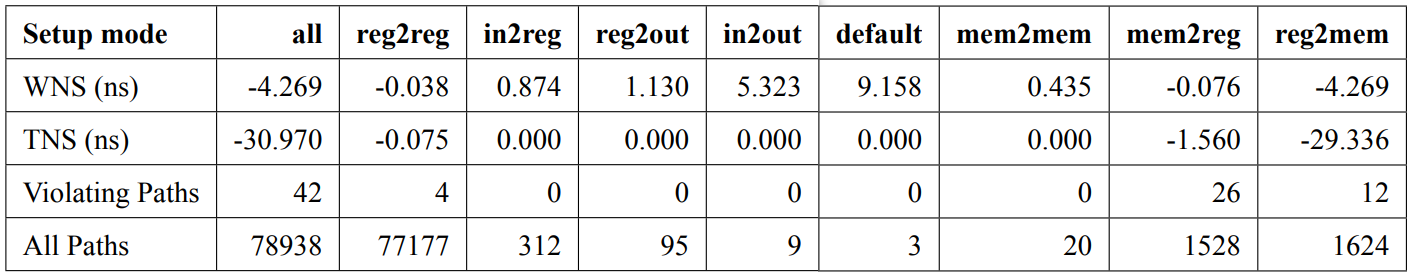
\includegraphics[width=0.7\linewidth]{assets/08/inittiming.png}
  \caption{initTiming时序检查报告}
  \label{fig:08-timing1}
\end{figure}

\begin{enumerate}
\def\labelenumi{\arabic{enumi}.}
\setcounter{enumi}{1}
\tightlist
\item
  \textbf{布局规划}
\end{enumerate}

在数字集成电路的设计过程中，floorplan 阶段通过迭代布局规划，可以在设计的早期阶段确保性能、功耗与面积三者之间达到更优的平衡。Floorplan 需要手工进行，人工确定芯片的面积大小、各个宏模块摆放的位置以及 IO 的顺序等。在本工程设计中，经过统计，工程设计中总门数为 170K，LeafCell 共计 223247 个，Pads 共计 121 个，Hard Macros 共计 31 个，总计面积 12.8mm2。综合考虑多方面的因素后，将版图的利用率（utilization）设置成 50\%，为了封装方便，将版图形状设计为四遍等长的正方形，最终版图尺寸定在了 4.8mm x 4.8mm，封装选择了 144 引脚的 QPF-144 封装。

在芯片设计中，确定宏模块的位置对布局质量至关重要，影响时序检查和布线拥塞。宏模块面积较大，布局后会影响标准单元分布和信号路径，进而影响时序结果。宏模块的Pin数量和周围标准单元密度影响布线资源，可能导致布线拥塞。这些因素都需要在布局宏模块时考虑。

针对因素规划宏模块布局：将含模拟信号的PLL置于右上角以缩短走线并减少数字干扰，设禁止区；数模相邻区设Guard Ring隔噪并符合DRC；加输入Buffer确保信号正常驱动根节点。对于 RAM 等 PIN 较多的模块，边缘需要留出足够的布线空间进行布线，因此通过对齐、旋转等操作，将其中的 PIN 尽量面向中部的 SOC 数字逻辑区域，并添加禁止区域，减少布局密度，提供布线通道，从而增加布通率。图\ref{fig:08-macro-place}展示了经过上述调整的宏模块布局。

\begin{figure}[htbp]
  \centering
  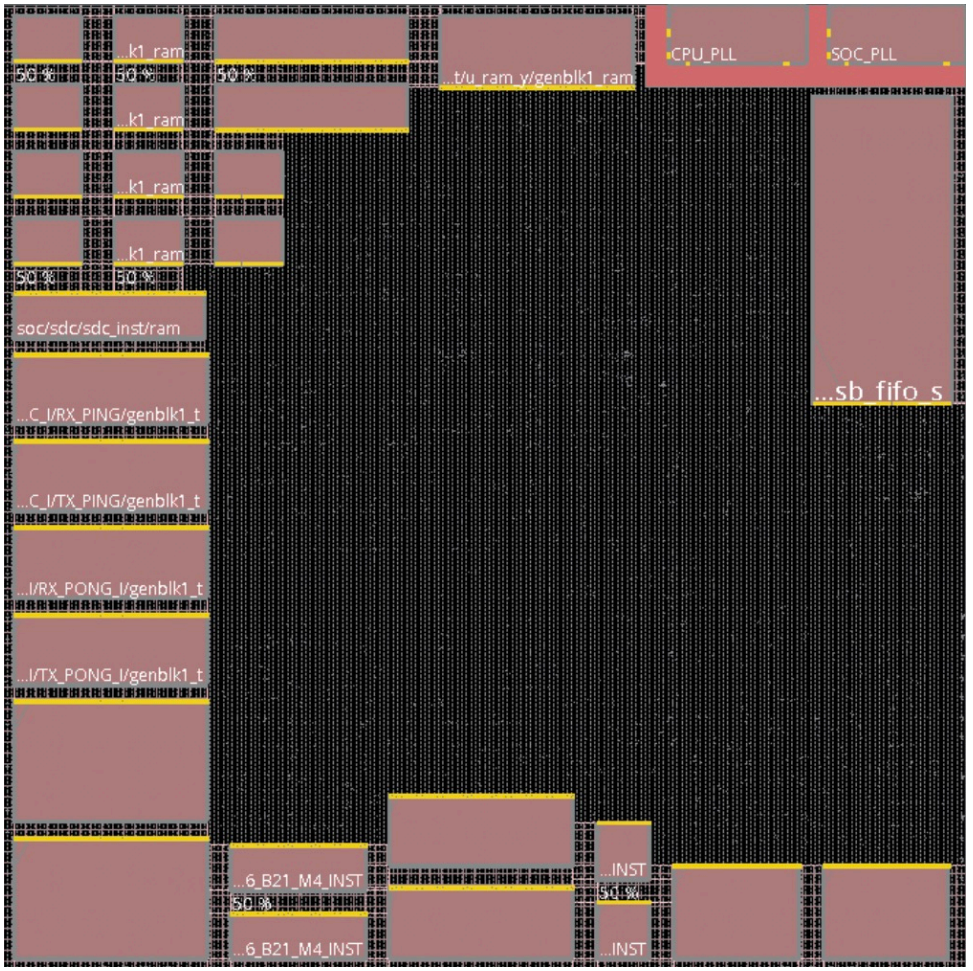
\includegraphics[width=0.7\linewidth]{assets/08/macro_place.png}
  \caption{宏模块布局结果}
  \label{fig:08-macro-place}
\end{figure}

IO 布局是 floorplan 的一个重要组成部分，在设计过程中将 IO 的坐标写入到文件中，从而将摆放 IO 加入到自动化流程中来。在自动化脚本中需要指定芯片的尺寸、IO 填充单元的位置，并添加 IO 填充器以确保 IO 区域的完整性和电气特性。通过 `floorPlan`命令设置了初始芯片的尺寸和位置参数，通过 `loadIoFile`命令加载了 IO 布局文件，并且通过 `addIoFiller`命令在芯片的不同边添加了 IO 填充单元，以确保 IO 区域的填充。此外，IO 的布局需要参考内部的布局与封装，避免封装线交叉，并将同一类的 IO 放置在一起。添加了 IO 布局的版图效果如图\ref{fig:08-IO-place}所示：

\begin{figure}[htbp]
  \centering
  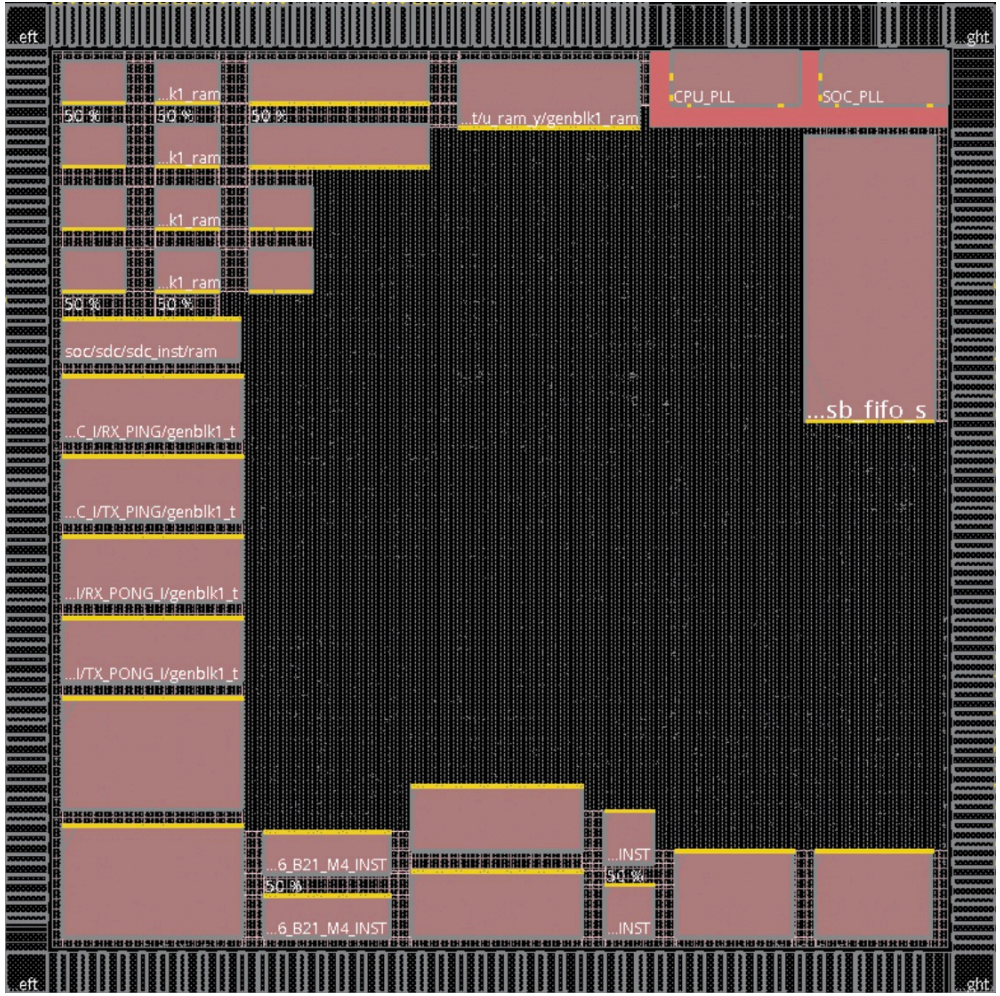
\includegraphics[width=0.7\linewidth]{assets/08/IO_place.png}
  \caption{IO布局结果}
  \label{fig:08-IO-place}
\end{figure}

对于供电部分，四条边对数字供电和模拟供电均提供了至少两组供电 IO pin，以保证内部标准单元得到充分供电的同时降低电压降（IR Drop）和电迁移（EM）。在设计过程中采用了环（ring）和条带（stripe）的方式，对电源和地网络进行优化。这些操作针对所有的电源域进行，以确保整个设计中电源和地的分布均匀、有效，减小 IR Drop，同时也考虑到了电迁移的影响。由于库中没有带定义的多电源的工艺文件，因此不能通过多电压域的方式降低功耗。添加电源的布局版图效果如图\ref{fig:08-power-place}所示：

\begin{figure}[htbp]
  \centering
  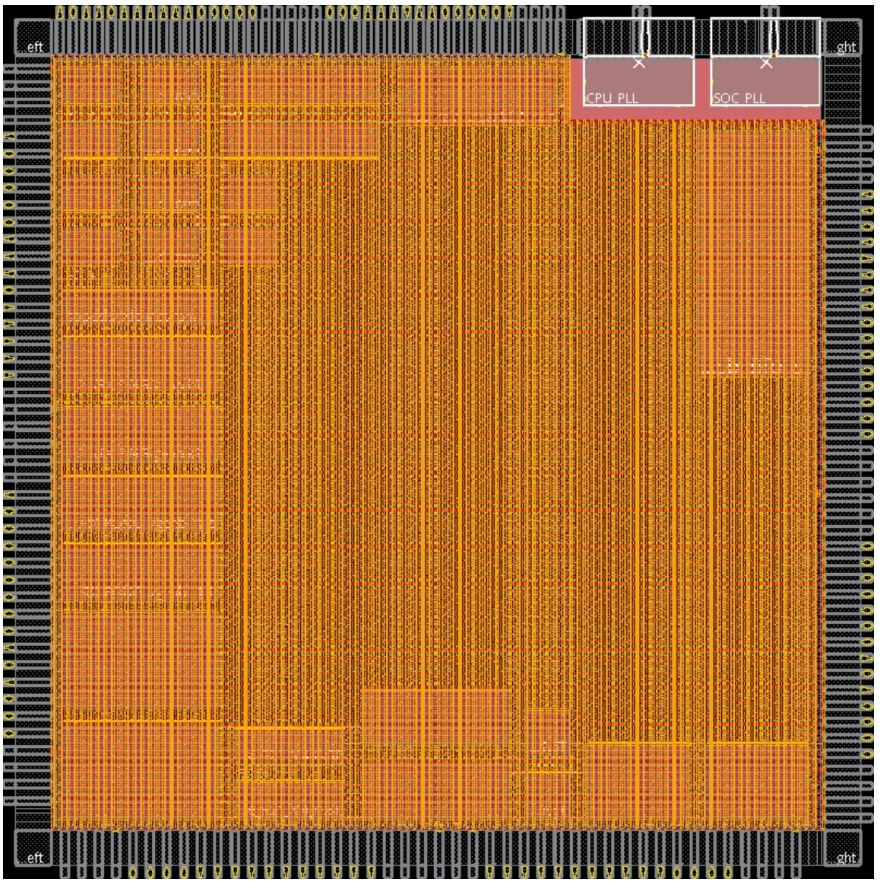
\includegraphics[width=0.7\linewidth]{assets/08/power_place.png}
  \caption{电源规划结果}
  \label{fig:08-power-place}
\end{figure}

在完成初步的 floorplan 设置之后，通过执行电源验证（Power Early Analysis）、设计规则检查（DRC）和连接性验证等步骤，确保设计满足制造要求。在 DRC 检查过程中，约 4-5 处电源条带由于宏模块的隔断或者宏模块内部结构影响的原因产生了 DRC。经过分析是极个别电源金属层未能成功联通以及宏模块内部金属层带来 DRC 要求的原因，因此可以直接删除掉产生 DRC 的金属图形，并不会对整体供电带来显著影响。以上各步骤完成了布局规划阶段的设计，并确保设计在多个 view 下的时序收敛和一致性。布局规划阶段完成了对芯片尺寸的确定、宏模块与 IO 引脚的布局以及电源网络生成。目前为止所进行的操作已经基本确定了芯片的形状与规划，接下来是标准单元布局部分

\begin{enumerate}
\def\labelenumi{\arabic{enumi}.}
\setcounter{enumi}{2}
\tightlist
\item
  \textbf{布局}
\end{enumerate}

布局（Placement）阶段是在布局规划的基础上为标准单元找到合适的位置并进行优化。EDA 工具会根据宏单元的摆放位置、时序约束文件和用户的特殊设定自动完成布局。布局的主要目标包括：优化 PPA（功耗、性能、面积），实现合理的全局拥塞（global congestion）和局部拥塞（local congestion）控制，避免出现高的引脚密度区域和热点区域，确保合理的时序结果，并满足 DRC（设计规则检查）要求。以下详细描述了布局阶段的具体步骤及对应的代码实现。

在粗略布局（Coarse Placement）阶段，Innovus工具根据时序、拥塞和多电压域进行标准单元的初步摆放。粗略布局阶段的主要目标是快速生成一个初步的布局结果，用于评估和分析全局拥塞情况，优化全局和局部拥塞，以确保在布局过程中，全局和局部的单元密度保持均匀，避免过度拥塞的区域，提高布局的整体效果。

在初步优化（Preliminary Optimization）阶段，工具将对时序、面积、拥塞和功耗进行优化。该阶段通过启用数据到数据检查和 useful skew，可以有效减少时序上的不确定性，提高设计的时序质量。这些优化设置确保了设计在时序、功耗和面积方面的均衡优化。

有些单元对于当前设计来说面积过大，或者时序表现较差，为了避免不适合当前设计的单元被意外使用，提高设计的可靠性，加快时序收敛，减小布局面积，需要对特定类型的单元进行排除设置。通过设置排除单元（setDontUse）命令，可以防止时钟缓冲器和其他特定单元在布局中被使用，从而提高设计的稳定性。

为了提高布局的时序精度，需要设置时钟不确定性和交互式约束模式。通过设置时钟路径上的不确定性，可以进一步优化时序性能，确保时钟信号在不同路径上的延迟保持一致，从而提高设计的整体时序质量。为了保持软 IP 端口的一致性，在布局过程中需要保持特定端口的稳定性，防止其被意外更改。可以人工定义 keepPortList，通过读取端口列表并将其设置为不可更改状态，确保这些关键端口在布局过程中不会被移动或修改：

在布局过程中，为确保 SDRAM 寄存器时序的性能，将和 SDRAM 模块相关的寄存器进行集中预放置。这一步骤通过提前放置 SDRAM 寄存器，确保其位置靠近 SDRAM的宏模块，有助于后续布局时序优化，从而减少后期调整的工作量。

为了进一步提升 PPA（功耗、性能、面积），需要进行特定单元的优化操作。通过替换特定单元，进一步优化设计的功耗和性能，这些优化操作有助于在不影响设计功能的前提下，最大限度地提升设计的效率和性能。此外，还需要修复设计中的最大延迟问题，以确保设计的时序性能达到要求。可以通过加载人工定义的路径组的配置脚本，修复设计中的最大延迟问题。

place\_opt\_design 命令可以优化设计的布局，以提高时序和减少拥塞。布局优化步骤可以显著提升设计的整体性能，并减少后续设计阶段的调整工作量。为了确保设计的完整性，增加高低电平拉电阻。通过增加高低电平拉电阻，可以防止浮动节点，提高设计的电气稳定性。

最后，对设计进行设计规则检查与时序检查，得到布局结束后的时序报告与DRC报告，时序报告中有 113 条违约路径，DRC 全部通过。将会在下面的时钟树综合与布线阶段对时序违约路径进行处理。布局完成的版图如图\ref{fig:08-place}所示。

\begin{figure}[htbp]
  \centering
  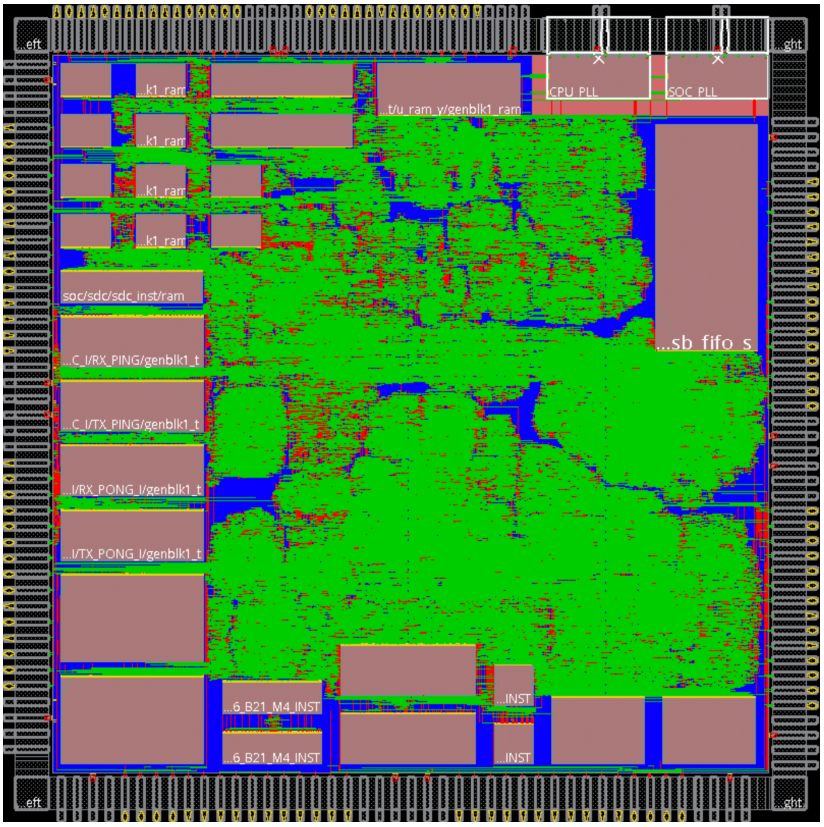
\includegraphics[width=0.7\linewidth]{assets/08/place.png}
  \caption{最终布局结果}
  \label{fig:08-place}
\end{figure}

\subsubsection{时钟树综合（CTS）阶段}\label{sec:08-verification-and-implementation-016}

在时钟树综合（CTS）阶段，目标是构建一个高效且稳定的时钟网络，以满足设计的时序要求。该阶段包含了多个关键的配置和策略，确保时钟信号在整个芯片上的分布均匀且准确。首先，加载放置阶段完成后的设计数据库，为 CTS 步骤做好准备。为提高布局质量，对特定库单元（如 PO16 和 PB16），通过 dbAddCellObs 命令在 M1 至 M6 层添加障碍物，避免布线时穿越这些关键单元，从而提升设计的可靠性和性能。为了优化时钟网络的设计，使用 set\_ccopt\_property 命令设置了一系列属性，包括启用反相器、定义反相器单元列表以及时钟网络的非默认规则（NDR）。特别地，定义了两种类型的时钟网络路径------主干（trunk）和叶子（leaf），并分别为它们设置了优先布线层和保护层策略，确保时钟信号的传输效率和稳定性。

启用反相器并定义反相器单元列表，优化时钟分布。添加一个名为 clock\_2w2s\_-shield的非默认规则（NDR），以生成必要的过孔并设置金属层之间的间距和宽度倍数。这些配置有助于提高时钟信号的传输质量和电气性能。随后，创建了两种时钟布线类型：clock\_trunk 和 clock\_leaf，并为它们分别设置了优先布线层和保护层策略，以确保时钟信号在主干和叶子路径上的高效传输。通过 generateVias 命令生成了必要的过孔，以确保不同金属层之间的电气连接。此外，通过 create\_ccopt\_clock\_tree\_spec 命令和source ccopt.spec 操作，根据预定义生成并应用了时钟树的设计，为时钟网络的构建提供了具体指导。

这些步骤确保了在时钟树构建过程中，各金属层之间的电气连接得到充分保证。通过预定义时钟树规范可以有效地指导时钟树的构建，确保时钟网络的结构合理性和性能。在 CTS 执行之前，需要对特定的时钟网络进行了微调，例如，为 SDRAM 的时钟网络创建了一个专有的时钟偏移组，并调整了时钟不确定性设置，以满足严格的时序要求。这些设置包括移除和创建新的时钟偏移组、忽略特定引脚类型、设定插入延迟、调整时钟不确定性等。这些微调确保了时钟信号在特定路径上的延迟和偏差都在可控范围内，从而满足设计的严格时序要求。

接下来，通过执行 ccopt\_design 命令构建和优化时钟树。该命令是 CTS 过程的核心步骤，涉及时钟网络的构建、优化和验证，以确保整个设计满足时序要求，同时保持功耗和面积的优化。在时钟树构建和优化完成后，通过 optDesign -postCTS -setup -hold命令进行 postCTS 优化，进一步调整设计以满足所有的设置和保持时序要求。同时，使用 addFiller 命令添加填充单元，以优化芯片内的空间利用率并减少制造过程中的问题。

在这些步骤中，通过 setOptMode 命令设置了保持修正单元列表，以确保在保持时序优化过程中使用适当的单元。接着，通过 setAnalysisMode 和 setOptMode 命令，设置了芯片内变量分析模式、保持目标余量以及有用偏斜选项。这些设置有助于提高设计的时序裕量和可靠性。另外，通过 setDontUse 命令，限制了某些单元的使用，以防止这些单元影响设计的性能和稳定性。最后，通过保留软 IP 端口的设置，确保在优化过程中不会修改关键端口。执行 optDesign -postCTS -setup -hold 命令，进行后 CTS 优化，确保所有的设置和保持时序要求都得到满足。最后，通过 setFillerMode 和 addFiller 命令，添加填充单元，以保证 density 并减少制造过程中的 DRC 问题。

时钟树综合（CTS）阶段通过一系列优化和配置步骤，确保时钟信号在整个芯片上的分布均匀且满足设计的时序要求。通过加载设计数据库、添加障碍区域、设置优化属性、生成过孔、创建时钟树规范、微调时钟网络、构建和优化时钟树、以及后续的优化和填充单元添加，最终实现了高效且稳定的时钟网络设计。postCTS 的时序检查报告如表\ref{fig:08-PostCTS}所示，违约路径 12 条，分别是 8 条 reg2out 和 4 条 in2out 路径。这些问题将会在后续时序修复时进行处理。

\begin{figure}[htbp]
  \centering
  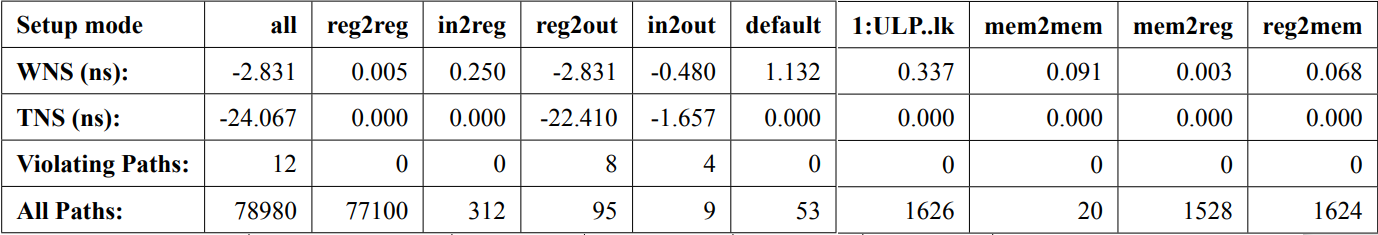
\includegraphics[width=0.7\linewidth]{assets/08/PostCTS.png}
  \caption{PostCTS时序检查报告}
  \label{fig:08-PostCTS}
\end{figure}

时钟树综合之后的结果如图\ref{fig:08-PostCTS-res}所示。

\begin{figure}[htbp]
  \centering
  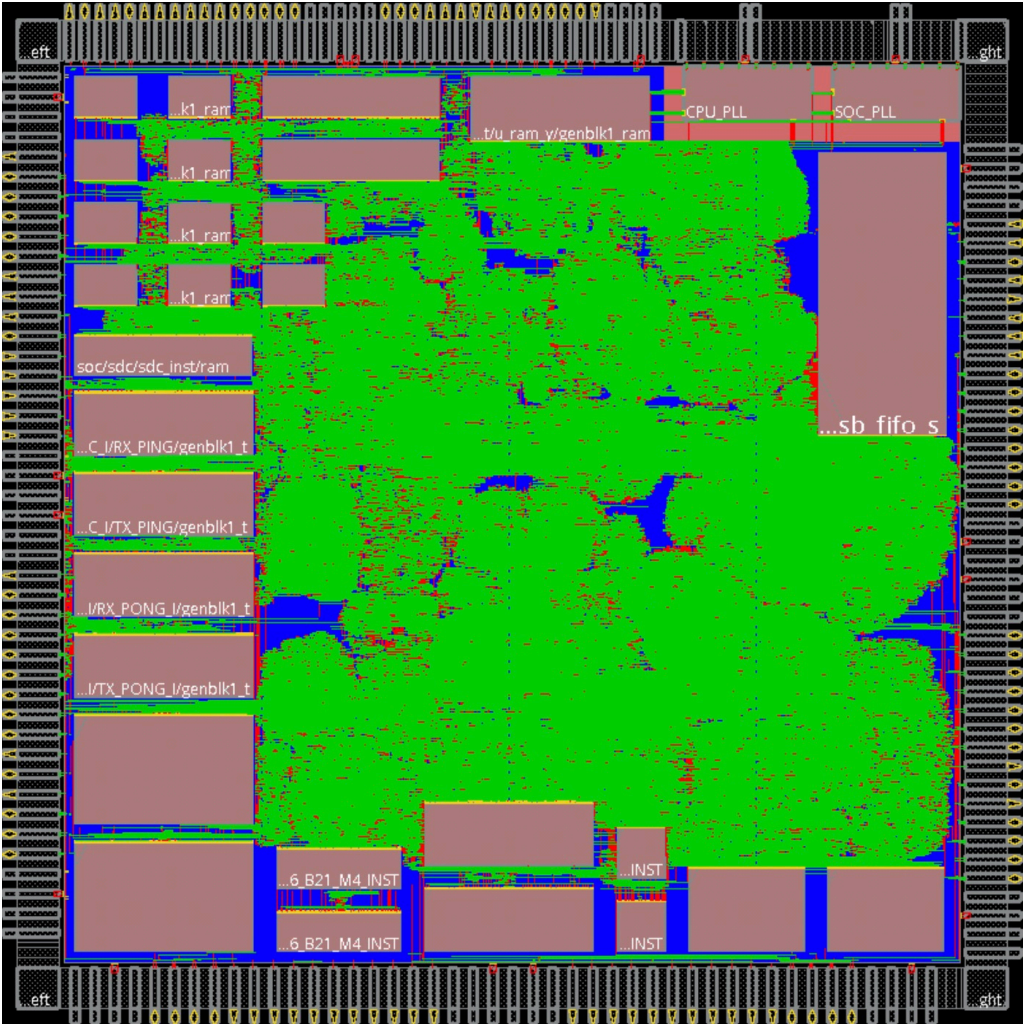
\includegraphics[width=0.7\linewidth]{assets/08/时钟树综合之后的版图.png}
  \caption{时钟树综合之后的版图}
  \label{fig:08-PostCTS-res}
\end{figure}

\subsubsection{布线规划}\label{sec:08-verification-and-implementation-017}

在布线阶段，目标是构建高效的信号传输路径，同时解决信号完整性（SI）和天线效应等潜在问题。此阶段的关键在于通过一系列精细的配置和优化策略，确保信号在整个芯片中的有效传输，同时满足时序、功耗和面积的要求。为了确保布线后的设计满足信号完整性和时序要求，使用了 setAnalysisMode、setDelayCalMode 和 setSIMode等命令对分析模式进行了详细配置。这包括信号完整性感知的时延计算以及信号完整性模式的设置，从而确保设计在最终验证时能够满足所有电气要求。这些配置通过精确的时延计算和信号完整性分析，确保了布线后的设计在所有操作条件下都能满足性能和可靠性要求。

在布线过程中由于 pin access 步骤，会出现设计规则（DRC）问题，需要通过 ECO（Engineering Change Order）流程进行修复。通过 ecoRoute 命令修复了 DRC 问题。在修复天线效应方面，特别指定了天线二极管单元进行修复，并通过设置setNanoRouteMode命令的不同选项来控制修复过程。这些命令通过修复设计规则检查问题和天线效应，确保了设计的制造可行性和信号完整性。

完成 ECO 布线后，进行了增量的后布线优化，通过 optDesign -postRoute -incr 命令对设计进行细微调整，以确保达到更优的时序性能。紧接着，执行 timeDesign -postRoute命令进行时序分析，生成最终的时序报告，确保设计满足所有设置和保持时序要求。

最终得到的时序报告如表\ref{fig:08-setup-time}所示，从表格中可以看出，经过优化与修复后的版图时序违约路径占比仅0.16\%。通过这一系列详细的步骤和配置，布线阶段确保了信号路径的有效性和电路设计的可靠性，实现了高性能、低功耗且面积优化的设计目标。

\begin{figure}[htbp]
  \centering
  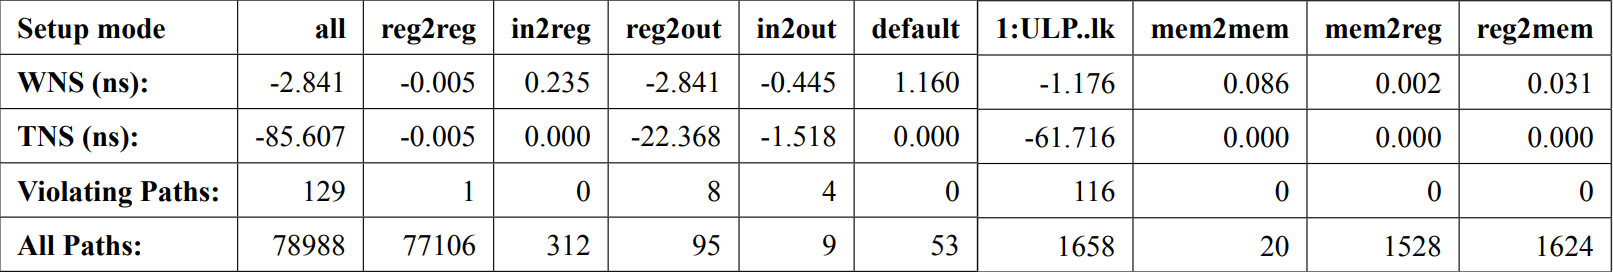
\includegraphics[width=0.7\linewidth]{assets/08/布线后的时序分析.png}
  \caption{布线后的时序分析}
  \label{fig:08-setup-time}
\end{figure}

经过上述步骤完成的版图如图\ref{fig:08-routed-layout}所示，可以交付到签核（signoff）阶段。

\begin{figure}[htbp]
  \centering
  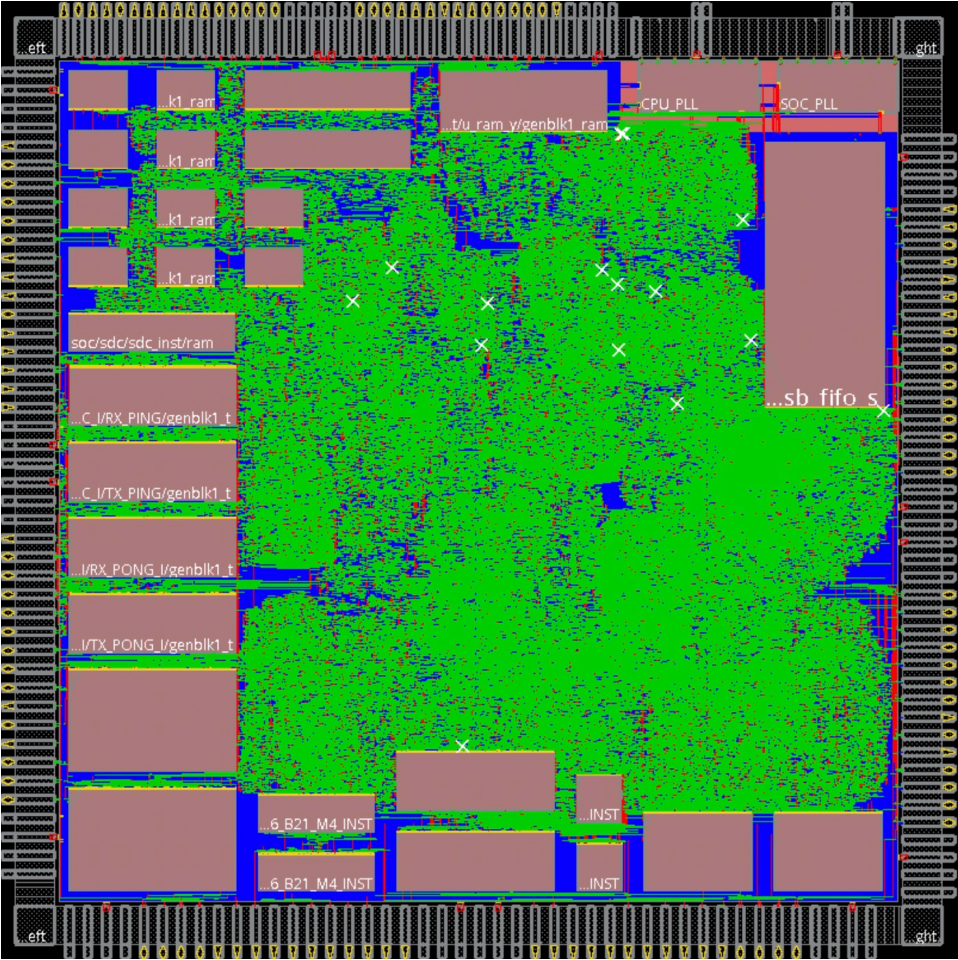
\includegraphics[width=0.7\linewidth]{assets/08/布线后的版图.png}
  \caption{布线后的版图}
  \label{fig:08-routed-layout}
\end{figure}

\subsection{芯片的验证与签核}\label{sec:08-verification-and-implementation-018}

芯片后端设计中的验证测试包括：时序验证、形式验证、物理验证和功耗验证。时序验证中，芯片需要在多模式多工艺角（MMMC）下实现时序收敛，达到设计频率要求。形式验证的目的是确保在布局布线之后芯片逻辑功能的准确性。物理验证主要包括设计规则检查（Design Rule Checking，DRC）、版图网表对比验证（Layout Versus Schematic，LVS）、天线效应验证和电气规则检查。功耗验证则包括静态功耗、动态功耗以及 IRDrop 的验证。当芯片的时序和功耗都达到设计指标，并且物理验证也满足工艺标准时，芯片就完成了流片前的签核。

\subsubsection{时序验证}\label{sec:08-verification-and-implementation-019}

时序验证包括两个阶段，分别是使用 Synopsys StarRC 工具对物理设计导出的版图进行 RC 抽取，随后使用 PrimeTime 工具对其进行时序分析并手工修复。RC 抽取是时序验证的第一步，它通过提取电阻（R）和电容（C）的信息，生成详细的寄生参数文件（SPEF），以便后续的时序分析。在 RC 抽取过程中，需要加载设计的LEF 文件和 DEF 文件，指定提取的目标模块和层次结构分隔符，配置寄生参数提取的详细选项，并并行处理多角（multi-corner）情况。func 功能模式下，本设计设置了 typ25、typ85、cmax125、cmaxm40、cmax0、cmin0、cminm40 这 7 个工艺角，可以基本涵盖在实际使用过程中的所有时序情况。时序分析与手工修复是通过 PrimeTime 工具对抽取的寄生参数进行详细的时序分析，并进行必要的手工修复，以确保设计满足所有时序约束。为了加速时序收敛，使用 PrimeTime 工具对所有工艺角并行进行静态时序分析，并给出报告。针对时序违例的工艺角也可以并行同时进行修复工作。对无法修复或者修复代价较高的违例路径采用人工手工修复的方式进行处理，利用好在布局阶段分散到版图各个位置的反向器等单元，实现最终时序的收敛。时序签核流程是一个较为漫长的过程，需要通过十几次迭代，并加入人工手工修复，最终使其达到时序签核标准。图 \ref{fig:08-timing-checkflow}为时序修复流程图，图\ref{fig:08-timing-report}展示了以 tt\_25 工艺角为例的经过多轮迭代修复后的时序报告，报告中显示，关键时序路径均得到了满足，时钟频率也达到了 140MHz 的设计要求。

\begin{figure}[htbp]
  \centering
  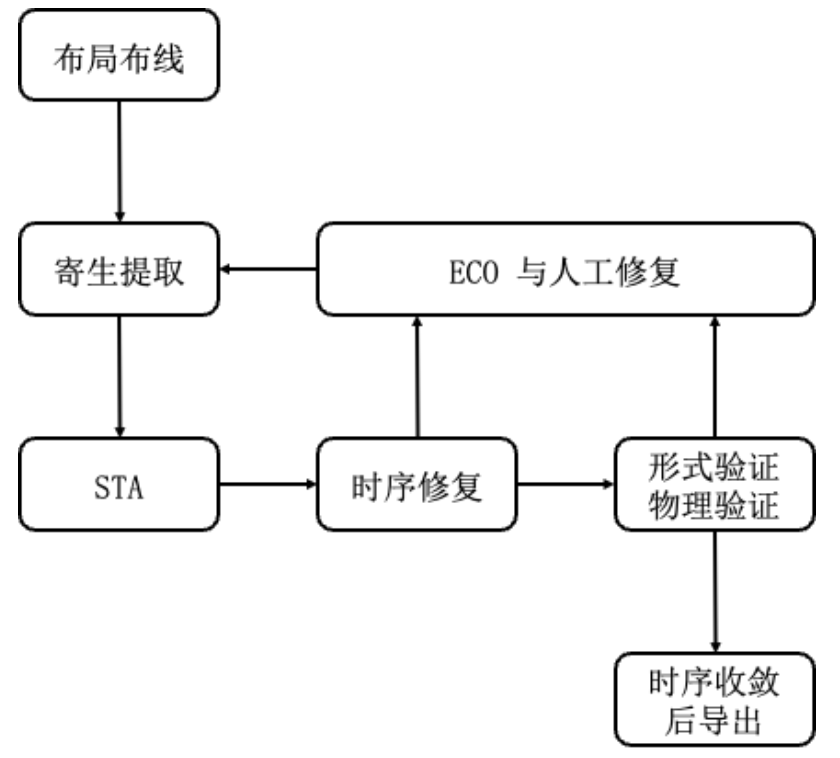
\includegraphics[width=0.7\linewidth]{assets/08/时序修复流程.png}
  \caption{时序修复流程}
  \label{fig:08-timing-checkflow}
\end{figure}

\begin{figure}[htbp]
  \centering
  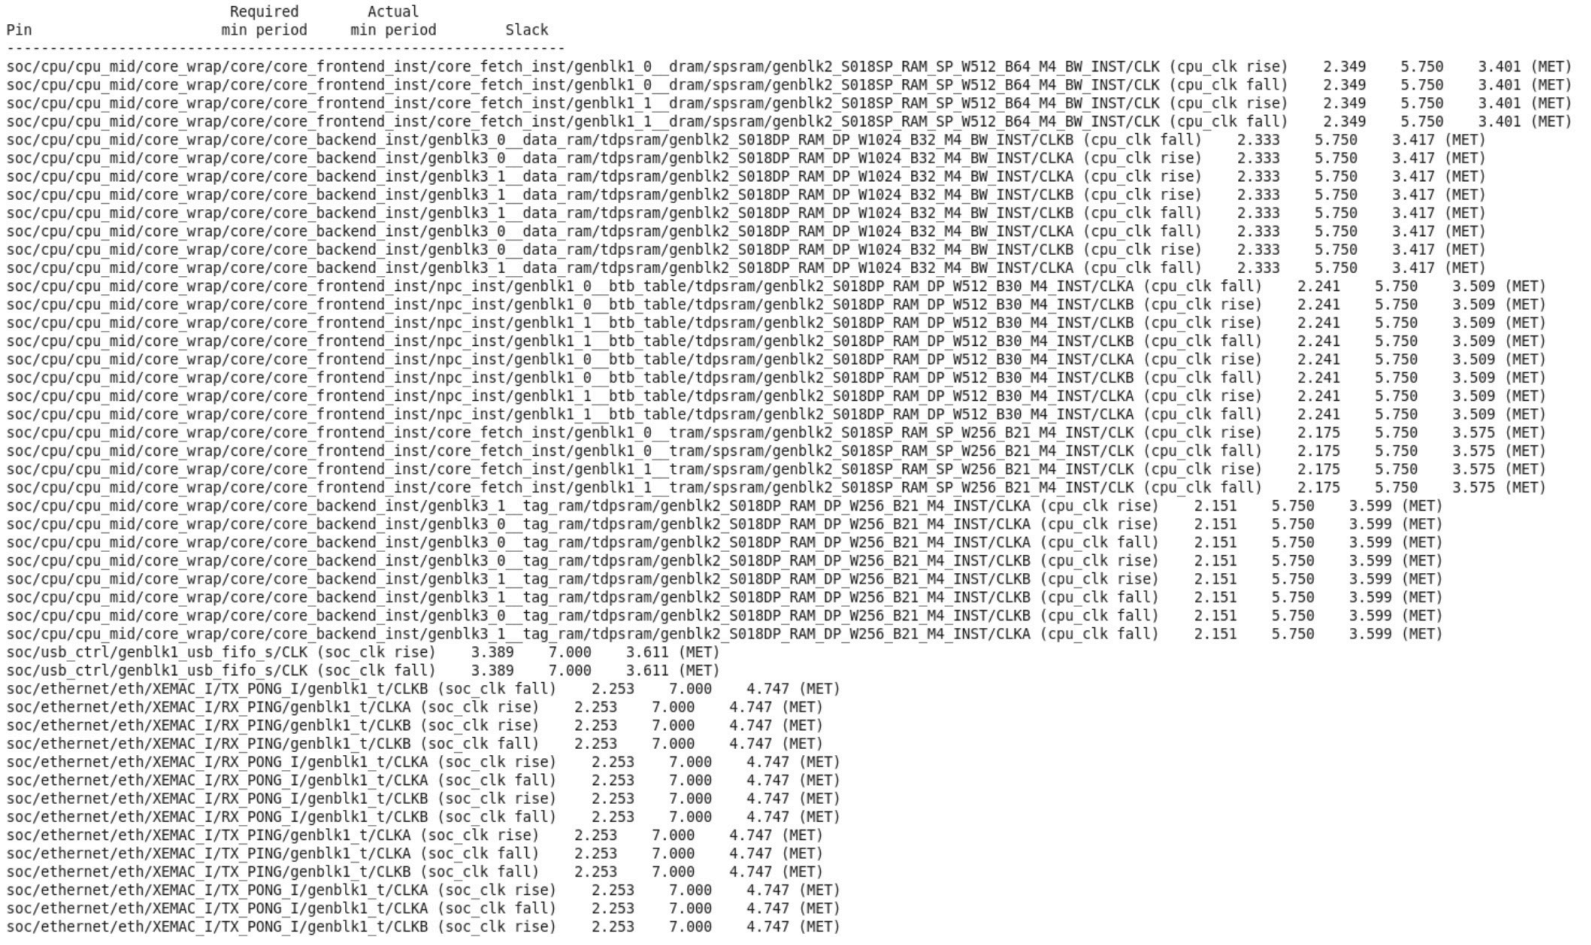
\includegraphics[width=0.7\linewidth]{assets/08/tt_25工艺角下的时序报告.png}
  \caption{tt\_25 工艺角下的时序检查报告}
  \label{fig:08-timing-report}
\end{figure}

\subsubsection{形式化验证}\label{sec:08-verification-and-implementation-020}

在芯片测试与验证章节中对形式化验证（即一致性验证）有所提及，这里主要针对综合后网表与布局布线后网表进行对比，旨在通过纯数学的方式分析两个网表的逻辑是否完全等价。与仿真相比，它的效率更高，会遍历所有的组合以保证逻辑等价，覆盖率高，获得结果速度快。采用Cadence LEC工具进行形式化验证，图\ref{fig:08-fm-flow}展示了形式化验证流程，图\ref{fig:08-LEC-res}展示了验证结果，从输出结果可以看出，形式化验证已通过。

\begin{figure}[htbp]
  \centering
  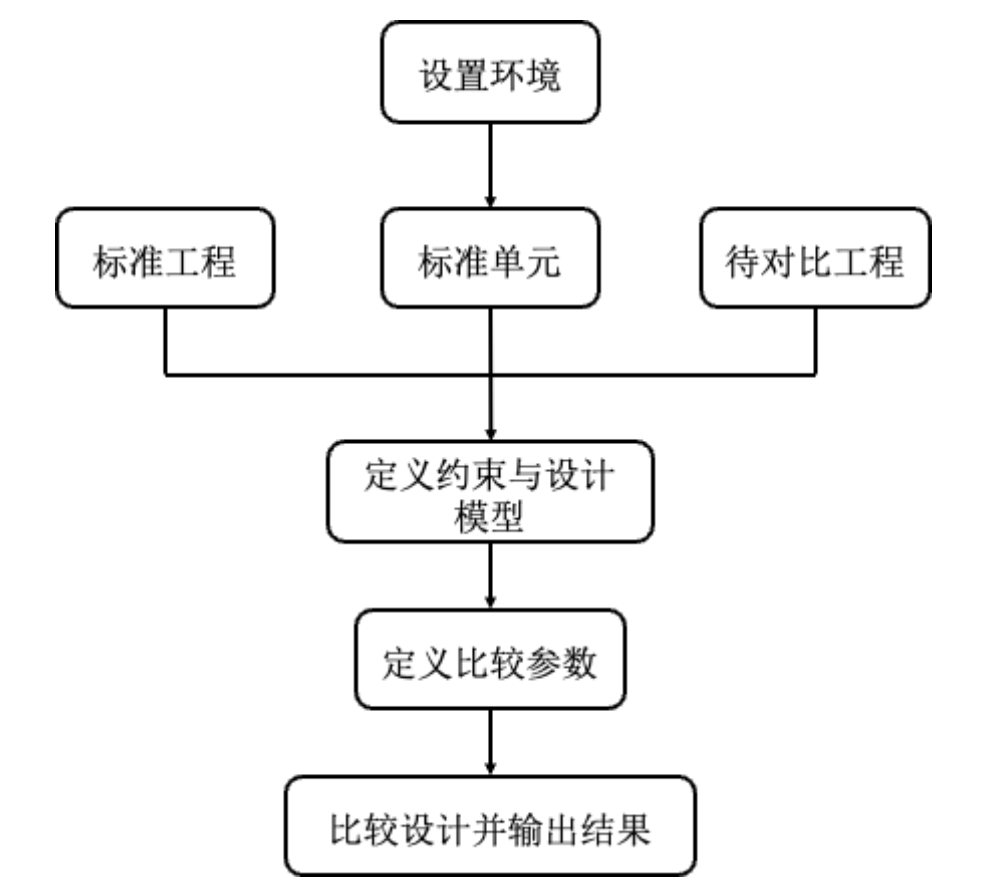
\includegraphics[width=0.7\linewidth]{assets/08/形式化验证.png}
  \caption{形式化验证流程}
  \label{fig:08-fm-flow}
\end{figure}

\begin{figure}[htbp]
  \centering
  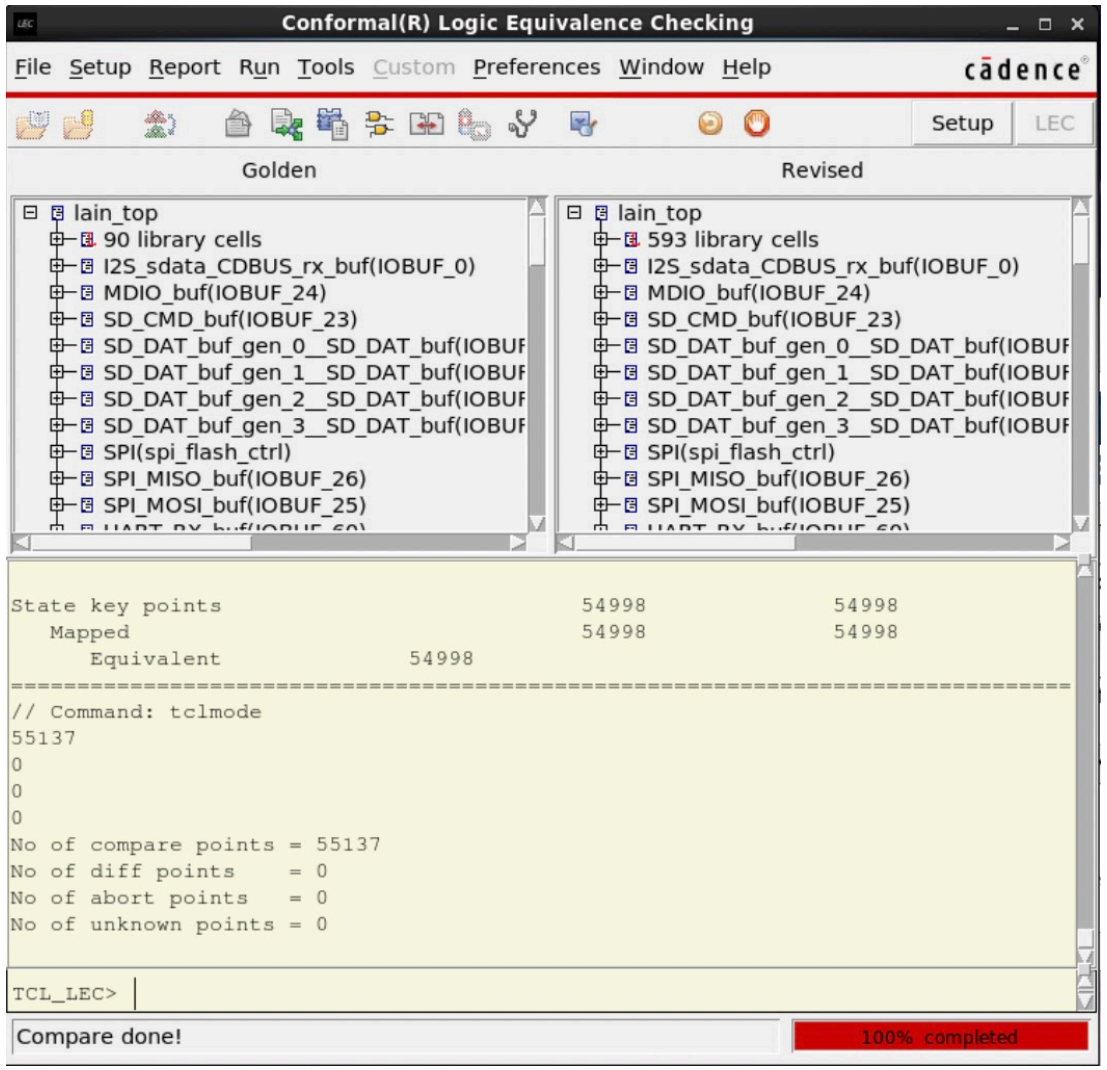
\includegraphics[width=0.7\linewidth]{assets/08/LEC验证结果.png}
  \caption{LEC验证结果}
  \label{fig:08-LEC-res}
\end{figure}

\subsubsection{功耗验证与电压降分析}\label{sec:08-verification-and-implementation-021}

本节描述使用 Voltus 工具进行功耗计算与电压降分析的过程。该分析针对经过时序修复后的版图，旨在验证其符合工艺和设计规范的功耗与电压降标准。

\begin{enumerate}
\def\labelenumi{\arabic{enumi}.}
\tightlist
\item
  \textbf{功耗计算}
\end{enumerate}

本小节详细介绍了使用 cadence voltus 工具对芯片功耗计算的过程。在数字电路设计中，功耗分为动态功耗与静态功耗两类。动态功耗主要由翻转功耗和短路功耗组成。

翻转功耗，也称为切换功耗，主要发生在电路中的电容充放电过程中，特别是当电路状态从 0 翻转到 1 或从 1 翻转到 0 时。翻转功耗的计算公式如下：

\[ P_{switching} = \alpha \cdot C_L \cdot V_{dd}^{2} \cdot f  \]

其中，\(\alpha\)是翻转频率，即每个时钟周期内电路节点状态翻转的概率，\(C_L\)是负载电容，\(V_{dd}\)是供电电压，f是时钟频率。翻转功耗与电路的工作频率、供电电压的平方和负载电容成正比，这意味着频率越高、电压越大、负载电容越大，翻转功耗也越大。

短路功耗主要出现在 CMOS 电路中，当输入信号变化导致 NMOS 和 PMOS 晶体管短暂同时导通时，会形成从电源到地的短路电流。在供电电压近似恒定时，观察时间 \(T\) 内的平均短路功耗可表示为：

\[ P_{short-circuit} = \frac{1}{T} \int_0^T V_{dd} \, i_{sc}(t) \, \mathrm{d}t  \]

其中 \(i_{sc}(t)\) 是瞬时短路电流，\(T\) 是观察时间。输入信号的上升和下降时间变长，通常会延长晶体管同时导通的时间，从而增加短路功耗；具体数值还取决于电流波形和开关活动。

静态功耗是数字电路中的一个重要概念，特别是在 CMOS 电路中，它指的是即使电路不进行任何切换操作时仍然发生的功耗。这种功耗主要由漏电流引起，包括多种不同形式。例如，即使晶体管关闭时，仍然存在一个微小的电流---称为漏电流---从源极流向漏极。此外，当晶体管的门电压低于其阈值电压时，会出现亚阈值漏电流，这是晶体管并未完全关闭时的低电平电流。随着晶体管尺寸的减小，这种漏电流成为功耗的一个显著部分。晶体管的栅极也可能出现电流泄漏，尤其是当其绝缘层变薄时，这些泄漏电流可以通过绝缘层到达通道或基底。此外，晶体管的源极和漏极与衬底之间的 PN 结在特定条件下也会产生泄漏电流。

动态功耗可以通过门控时钟技术、电源关断以及多电压域设计技术来实现优化。门控时钟技术（Clock Gating）是一种有效的动态功耗降低策略，它通过控制时钟信号的传输来实现。具体方法是，在时钟传输路径上加入逻辑门控制器，使得在不需要时钟信号的时段内，相关电路的时钟信号被切断，从而避免无意义的电路切换活动，减少功耗。这种技术可在模块级和门级上实施，能够精确控制各个部分的时钟活动，以优化功耗同时对系统性能带来极低的影响。电源关断技术（Power Gating）则主要针对降低静态功耗。该技术通过在电源与电路之间插入高阻值的开关（通常由一个或多个晶体管组成）来实现。在电路不活动时，通过断开其电源连接来消除漏电流，从而显著减少功耗。当电路需要恢复工作时，再次连接电源以恢复功能。电源关断允许按需动态地对芯片的不同部分进行电源管理，从而在整个系统级别实现功耗优化。多电压域设计（Multi-VoltageDesign）是一种设计同一芯片上具有多个操作电压的策略。通过为芯片上的不同功能块指定不同的操作电压，可以根据各部分的性能需求调整其功耗，使性能较不敏感的部分在更低的电压下运行以减少功耗，而性能关键的部分则可在较高电压下维持所需的性能。这种策略允许在不牺牲芯片整体性能的前提下，有效地降低功耗。如果功耗验证结果高于设计指标要求，可以通过上述手段对其进行改进，以符合设计指标。图\ref{fig:08-power-report}在展示了本设计在 tt\_85 工艺角下的功耗，功耗检查的报告中，芯片的总体功耗为 1.3W，小于设计指标 1.5W，因此符合设计要求。

\begin{figure}[htbp]
  \centering
  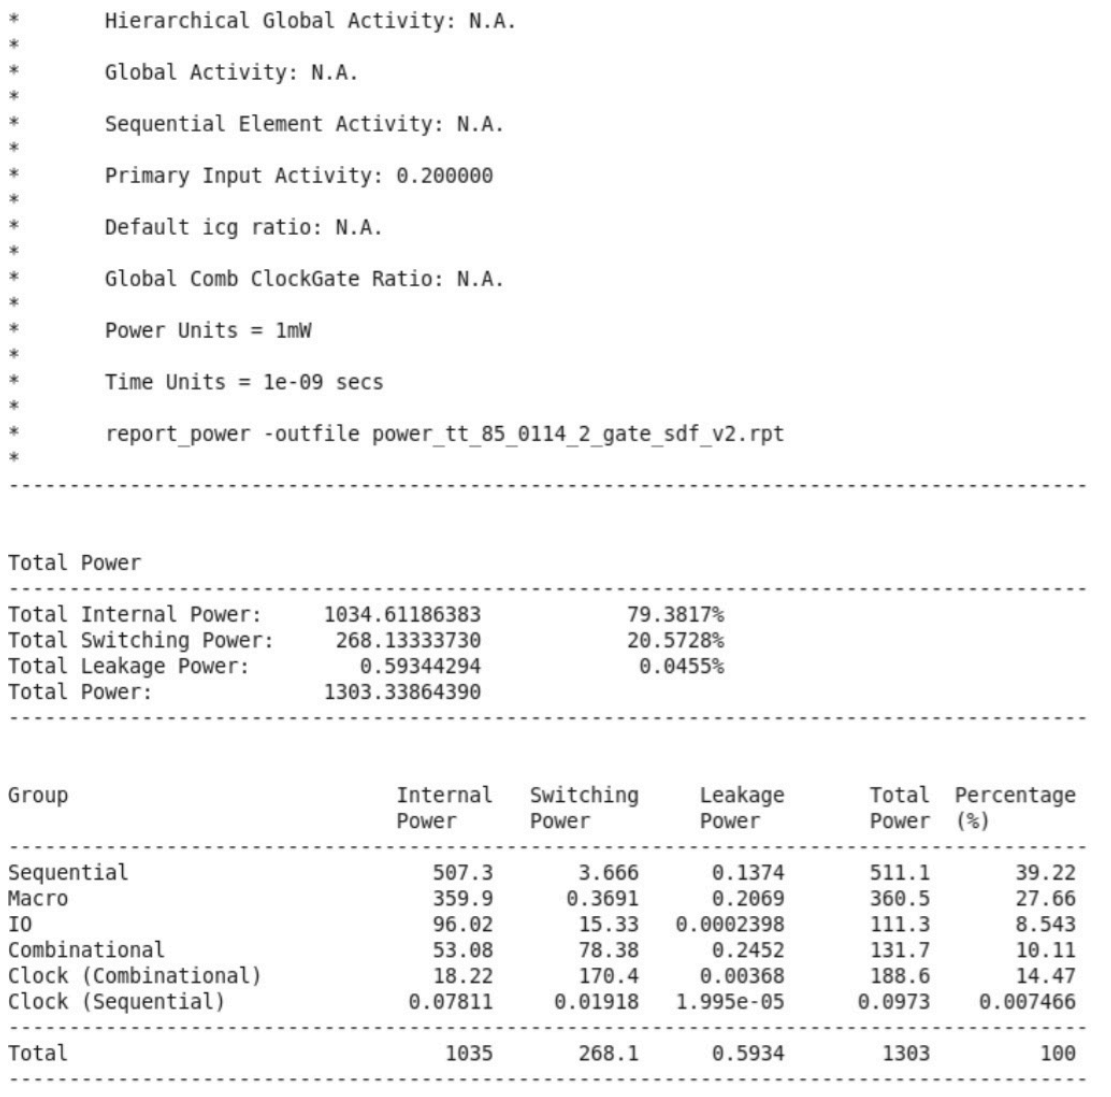
\includegraphics[width=0.7\linewidth]{assets/08/tt_85工艺角下的功耗.png}
  \caption{tt\_85 工艺角下的功耗报告}
  \label{fig:08-power-report}
\end{figure}

\begin{enumerate}
\def\labelenumi{\arabic{enumi}.}
\setcounter{enumi}{1}
\tightlist
\item
  \textbf{电压降分析}
\end{enumerate}

电压降分析是核心环节，用以确保芯片在所有工作条件下的电压稳定性。特别是对于高性能与大规模集成电路，电压降（IR drop）问题尤为关键。电压降指的是电源电压在经过电路传输路径时由于电阻和电感的存在而发生的降低。这种现象主要由电源和地线路径中的电阻引起，按照欧姆定律（V=IR），电流通过这些导体时会产生电压损失。在高频操作中，电感对电流变化的抵抗作用会进一步加剧电压降的问题。

电压降对电路性能和可靠性产生了显著影响。首先，电压降会降低晶体管的开关速度，这是因为晶体管的开关速度受到阈值电压的直接影响，进而导致整个电路性能的下降。在严重的情况下，电压降可能会导致电路部分功能失效，电压过低无法保证逻辑状态的正确性。此外，电压降还可能引起信号完整性问题，电压变化会影响信号的触发和时序，从而影响电路的整体稳定性和可靠性。

为了有效管理和缓解电压降带来的影响，有多种方式可以对其进行优化。通过增加电源和地线路径的金属层厚度，可以减少电阻，从而减轻电压降。设计均匀的电源网格有助于均匀分布电源电压，减少局部电压降。此外，去耦电容的引入可以稳定供电电压，在电源电压下降时提供必要的电荷以支持电路正常运行。实施多电压域设计通过将电路划分为多个独立的电压区域，并为每个区域优化电压级别，无需牺牲性能也可实现功耗优化。

考虑到设计与制造的可行性，代工厂对于电压降的指标是静态供电电压和地电压的总和不能超过 5\%，动态供电电压和地电压的总和不能超过 15\%。因此如果在签核阶段发现电压降不符合要求，需要重新回到布局规划阶段中的电源规划环节，通过调整电源网络密度以及部分重点区域的电源分布，以达到规定的设计指标。在本阶段，使用 Cadence Voltus 工具进行电压降计算。图\ref{fig:08-static-ir-drop}展示了经过 Voltus 工具计算的 VDDD 网络以及 GNDD 网络静态电压降数值。供电电压为 1.8V，从实验结果中可以看出，版图里面最差区域的电压是 1.756V，经过计算可以得出，本版图的静态电压降约为 2.5\%，满足设计要求，整体静态电压降经过计算符合设计指标。

\begin{figure}[htbp]
  \centering
  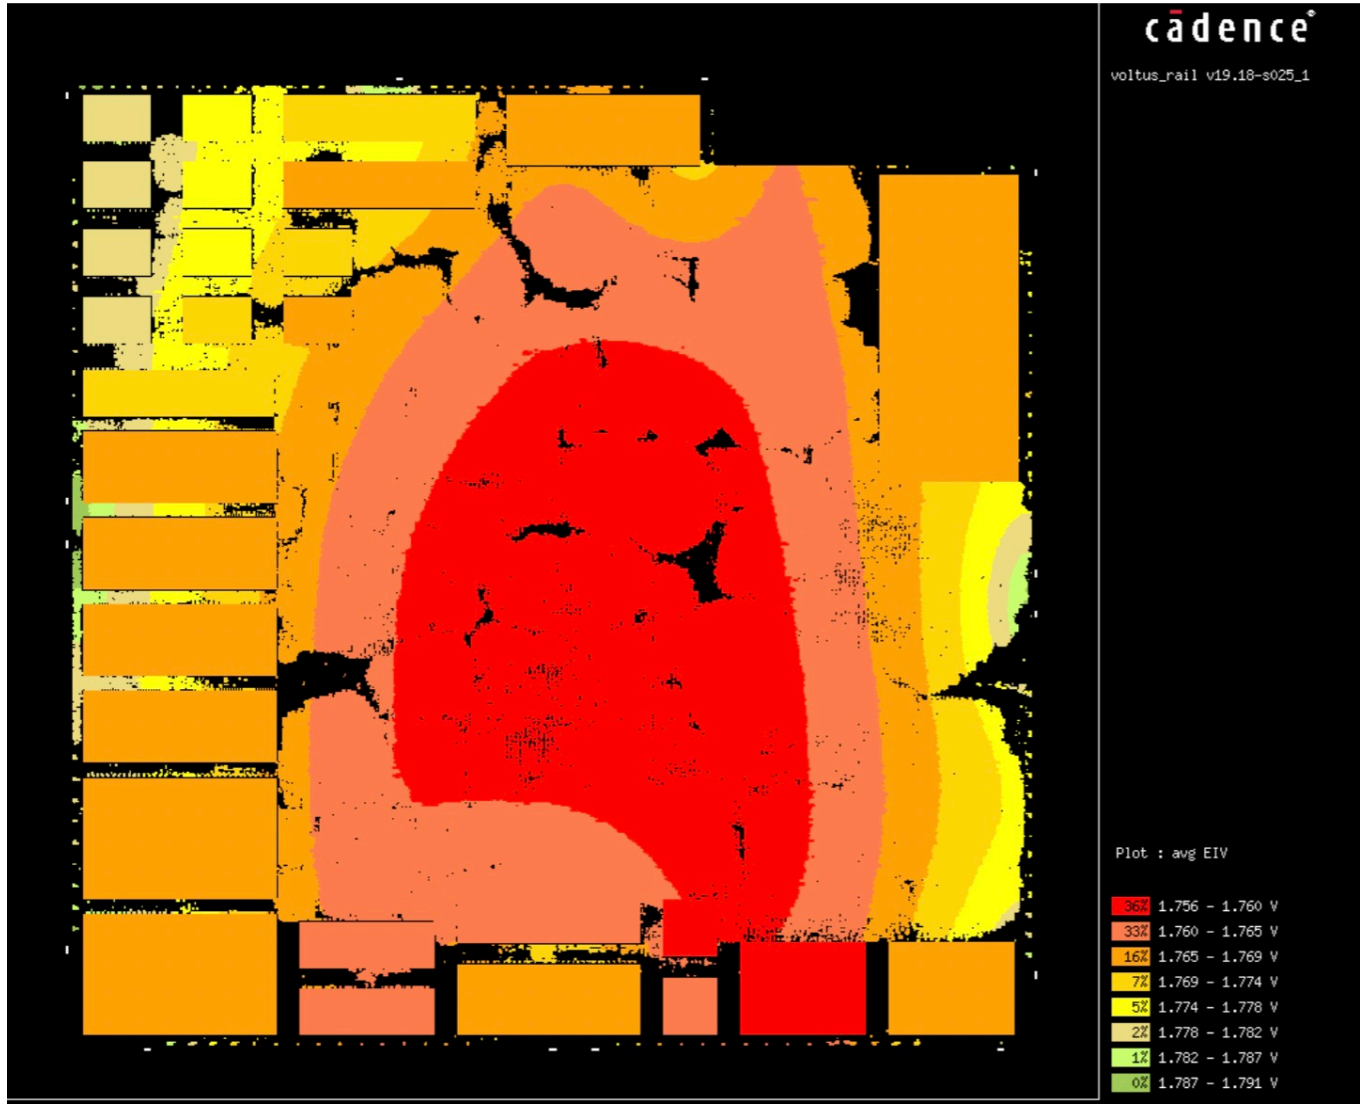
\includegraphics[width=0.7\linewidth]{assets/08/静态电压降分析结果.png}
  \caption{静态电压降分析结果}
  \label{fig:08-static-ir-drop}
\end{figure}

对于动态电压分析，同样通过 Cadence Voltus 工具进行分析计算，具体过程便不再赘述。图\ref{fig:08-dynamic-ir-drop}展示了动态电压降的分析结果，动态电压降为 8.3\%，满足设计要求。静态电压降与动态电压降均满足设计要求，因此本次设计的芯片可以通过功耗与电压降签核，满足设计标准。

\begin{figure}[htbp]
  \centering
  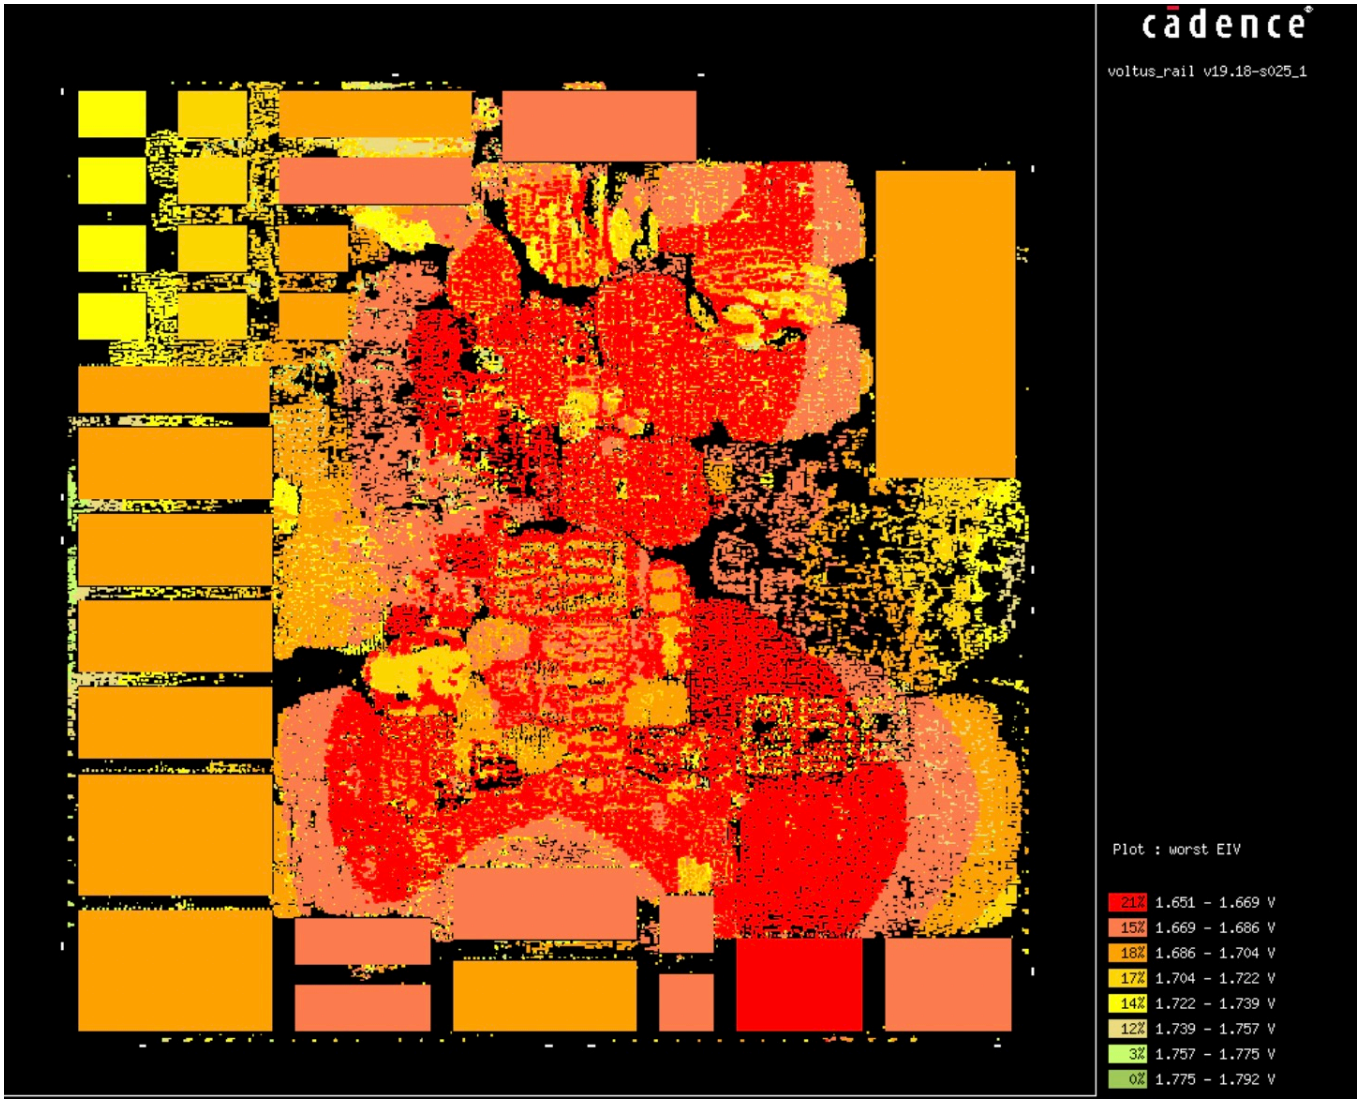
\includegraphics[width=0.7\linewidth]{assets/08/动态电压降分析结果.png}
  \caption{动态电压降分析结果}
  \label{fig:08-dynamic-ir-drop}
\end{figure}

表\ref{fig:08-design-metrics}给出了处理器芯片设计参数与验证结果之间的对照，表中可以简明扼要地看出，最终交付流片的版图尺寸为5mm x 5mm，面积为 25mm2，工作频率为 140MHz，功耗为 1.3W，各项验证指标均满足了设计指标要求。

\begin{figure}[htbp]
  \centering
  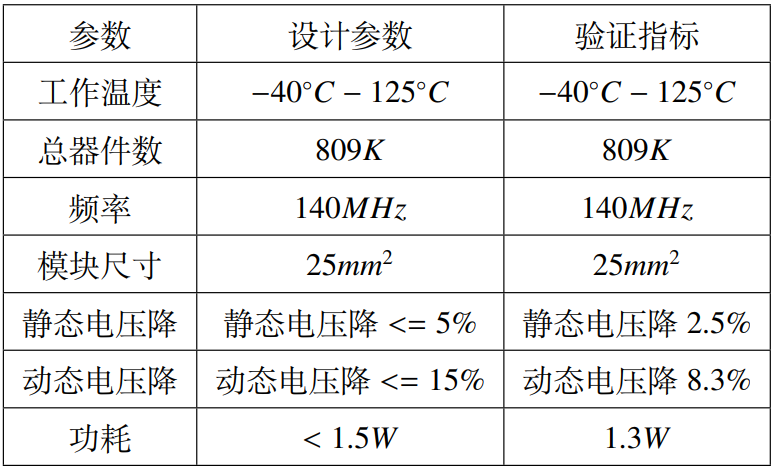
\includegraphics[width=0.7\linewidth]{assets/08/设计参数与验证指标对比.png}
  \caption{设计参数与验证指标对比}
  \label{fig:08-design-metrics}
\end{figure}

\subsection{物理验证}\label{sec:08-verification-and-implementation-022}

这里主要讲述使用Mentor Calibre数字后端工具进行LVS的过程。因为自动布局布线工具（简称为APR）所作的版图并不一定正确，因此需要通过LVS发现并改正APR工具布线的错误。LVS主要功能即为证明版图的逻辑与网表是一致的。可以分四部分进行表述：数据导出、v2lvs、Merge、LVS。

\begin{enumerate}
\def\labelenumi{\arabic{enumi}.}
\tightlist
\item
  \textbf{数据导出}
\end{enumerate}

导出APR EDA工具中的三个文件（Design.v.gz、Design.lvs.v.gz、Design.gds.gz）前，需确保设计在LVS（布局与原理图验证）和DRC（设计规则检查）中通过，保证没有短路和断开问题。导出的文件分别为两个网表和一个版图，代表设计的逻辑和物理信息。

% 代码语言：BookTcl
\begin{CodeBlock}[language=BookTcl]
#####ICC2：
verify_pg_nets

verify_lvs -max_error 100 -check_short_locator -check_open_locator \
           -ignore_floating_port -ignore_floating_net

check_lvs -checks {short open} -max_errors 1000

####INNOVUS：
verifyConnectivity -type all
\end{CodeBlock}

在ASIC后端设计过程中，确保填充单元（Filler）、电源和接地连接的正确性非常重要，特别是对于LVS检查。输出GDS文件时需要合并标准单元（merge stdcell），以确保完整性。

对应的命令如下

% 代码语言：BookTcl
\begin{CodeBlock}[language=BookTcl]
#update_names -nocase

##Netlist##
saveNetlist -excludeLeafCell ./data/Design.v.gz
saveNetlist -excludeLeafCell 
                           -excludeCellInst $pr_added_physical_cell \
                           -includePowerGround  \
                           -includePhysicalInst  \
                           -flattenBus  ./data/Design.lvs.v.gz

##GDSII#
##使用到的对应层的Mapfile
set map /home/PDK/smic/innovus/encStreamout_tm.map  
##需要merge standard cell的GDS,因为INN本身不带cell的
set GDS_LIST /home/PDK/smic/stdcellpath/stdcell.gds 

setStreamOutMode -virtualConnection false
deleteRouteBlk -all
deletePlaceBlockage -all
streamOut -uniquifyCellNames -mapFile $map -merge $GDS_LIST -unit 100  \
                             ./data/Design.gds.gz
\end{CodeBlock}

\begin{enumerate}
\def\labelenumi{\arabic{enumi}.}
\setcounter{enumi}{1}
\tightlist
\item
  \textbf{v2lvs}
\end{enumerate}

在数据导出阶段已经准备好了source的网表文件，需要使用v2lvs转换为工具识别的SPICE网表

% 代码语言：BookCShell
\begin{CodeBlock}[language=BookCShell]
set spice_name = Design   ;      #name of top
set final = /home/path/data/Design.lvs.v.gz
################################################
v2lvs \
      -v {$final} \
      -w 0 \
      -s  /home/PDK/smic/stdcell/cdl/std.cdl  \
      -s  /home/PDK/smic/Calibre/LVS/empty_subckt.sp  \
      -o  ./${spice_name}.spi
\end{CodeBlock}

\begin{enumerate}
\def\labelenumi{\arabic{enumi}.}
\setcounter{enumi}{2}
\tightlist
\item
  \textbf{Merge}
\end{enumerate}

在APR（本项目使用的Innovus）导出时已经合并（merge）了std的gds。如果不在APR工具导出时进行merge，也可以通过calibre导入进行merge。完成后需要在GDS中添加Dummy（虚拟单元，在布局中加入的占位符或虚拟组件）。

% 代码语言：BookCShell
\begin{CodeBlock}[language=BookCShell]
calibre -drc -hier -turbo 24 -turbo_litho 24 -hyper -nowait XXX.dmf \
        |& tee add_dummy.log
#############################
calibredrv -32 merge_all.tcl |& tee merge_all.log


#####################################merge_all.tcl
set L0 [layout create design.gds.gz -dt_expand -preservePaths]
set L1 [layout create Dummy.gds -dt_expand -preservePaths]

$L0 import layout $L1 FALSE rename -dt_expand -preservePaths
$L0 create ref design_topname design_dummy 0 0 0 0 1
$L0 gdsout design.final.gds.gz design_topname
\end{CodeBlock}

在Merge部分，需要先运行Fab（代工厂）提供的dummy添加脚本，设置好需要添加Dummy的层次。需要注意fab提供的脚本里的rule信息和提示，比如SMIC的dummy只会在Border区域（边界区域）里进行添加，需要确认好是否删除了所有的Blockage（布局时添加的不可通行区域），以及GDS导出时的Border区域是否满足要求。可以在Calibredrv里进行手动修改。接着将生成的dummy.gds与设计的gds进行merge，产生最终进行LVS验证所需要的文件。

\begin{enumerate}
\def\labelenumi{\arabic{enumi}.}
\setcounter{enumi}{3}
\tightlist
\item
  \textbf{LVS}
\end{enumerate}

可以通过命令行或者GUI的形式进行，这里以命令行的方式进行介绍：

% 代码语言：BookCShell
\begin{CodeBlock}[language=BookCShell]
#!/bin/csh -f

set top = design
set gds = /design_path/merge/design.final.gds.gz   #gds which have merged dummy 
set sch = /design/v2lvs/design.spi  #v2lvs from netlist

set gds_cell = ${ top }
set sch_cell = ${ top }
set block = ${top}

set rule_dir = /rule_path/rule/lvs/
set rule = XXX.lvs  #provide by fab
set hcell = /hcell_path/hecll

rm -rf runtime

calibre -lvs -hier -spice ${block} .layout.spice -turbo -hyper -hcell -64 \
${block}_${rule}.run | tee ${{block}_calibre.log
\end{CodeBlock}

运行完之后，可以使用dre打开版图，命令为calibredrv。最终得到图形\ref{fig:08-lvs-pass}，表示lvs通过。

\begin{figure}[htbp]
  \centering
  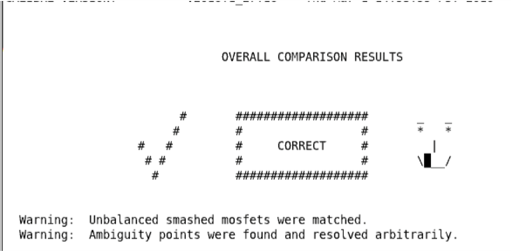
\includegraphics[width=0.7\linewidth]{assets/08/LVS验证通过.png}
  \caption{LVS通过}
  \label{fig:08-lvs-pass}
\end{figure}

\subsection{最终版图}\label{sec:08-verification-and-implementation-023}

最终针对EULA与LAIN两款CPU生成了两个版图设计，如图\ref{fig:08-layout1}与\ref{fig:08-layout2}。

\begin{figure}[htbp]
  \centering
  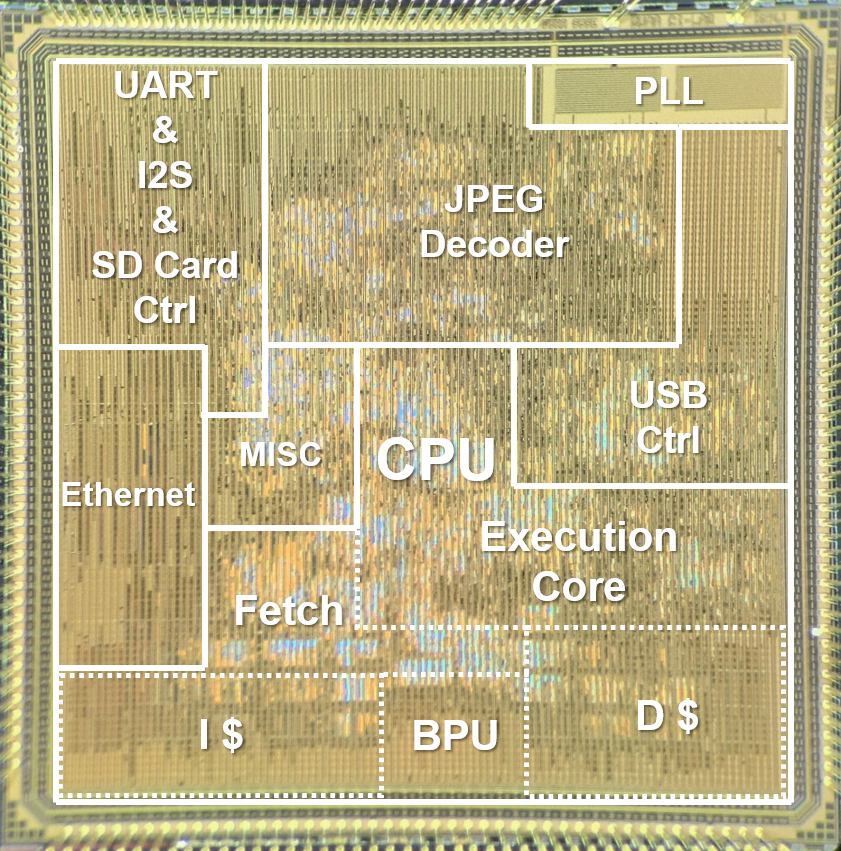
\includegraphics[width=0.7\linewidth]{assets/08/EULA芯片版图.png}
  \caption{EULA芯片版图}
  \label{fig:08-layout1}
\end{figure}

\begin{figure}[htbp]
  \centering
  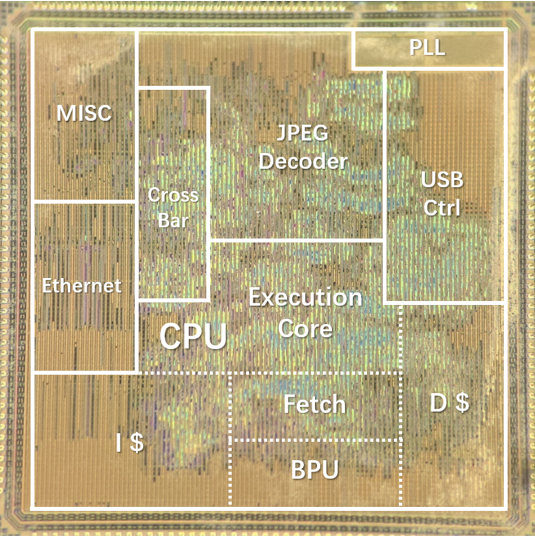
\includegraphics[width=0.7\linewidth]{assets/08/LAIN芯片版图.png}
  \caption{LAIN芯片版图}
  \label{fig:08-layout2}
\end{figure}
